% !TEX program = xelatex % (can also use "lualatex") 
\documentclass[12pt]{report}
\usepackage[fontsize=13pt]{scrextend}
\usepackage[a4paper,top=2cm,bottom=2cm,left=3cm,right=2cm]{geometry}
% \usepackage{svg}
\usepackage{tgtermes}
\usepackage{fontspec}
\usepackage{biblatex}
\usepackage{url}

\addbibresource{sections/ref.bib}
\usepackage{tikz}
\usetikzlibrary{shapes, arrows, positioning, shapes.geometric}
\usepackage{pgfsys}
\usepackage{transparent}
\usepackage{graphicx}
\setmainfont{Times New Roman}
\usepackage{eso-pic}

\usepackage{fancyhdr}
\usepackage{lastpage}
\usepackage{tabularx}
\usepackage{amsmath}

\usepackage{anyfontsize}
\usepackage{float}
\usepackage{titlesec}
\usepackage{listings}
\usepackage{lscape}
\linespread{1.5}
\usepackage{hyperref}
\usepackage{longtable}
\hypersetup{
    colorlinks,
    citecolor=black,
    filecolor=black,
    linkcolor=black,
    urlcolor=black
}
\usepackage{subcaption}


\lstset{
    basicstyle=\small\ttfamily, % Small font size
    numbers=left,
    frame=single,
}
\usepackage{pgfplots} % Required for the TikZ figure
% \usepgfplotslibrary{external}
% \tikzexternalize % Create a folder named 'saved-figures' first!
\pgfplotsset{compat=1.17} % Ensure compatibility with the latest version of pgfplots
\usepackage[utf8]{inputenc}
\usepackage[acronym, toc]{glossaries} % Load gói glossaries
\makeglossaries % Lệnh bắt buộc để tạo index
\loadglsentries{sections/list-of-abbreviations}
% Định nghĩa màu giống VS Code
\definecolor{codegreen}{rgb}{0,0.6,0}
\definecolor{codegray}{rgb}{0.5,0.5,0.5}
\definecolor{codepurple}{rgb}{0.58,0,0.82}
\definecolor{backcolour}{rgb}{0.95,0.95,0.92}

\lstdefinestyle{mystyle}{
    backgroundcolor=\color{backcolour},   
    commentstyle=\color{codegreen},
    keywordstyle=\color{magenta},
    numberstyle=\tiny\color{codegray},
    stringstyle=\color{codepurple},
    basicstyle=\ttfamily\footnotesize, % Font chữ code nhỏ gọn
    breakatwhitespace=false,         
    breaklines=true,                 % Tự xuống dòng nếu code quá dài
    captionpos=b,                    % Caption nằm dưới
    keepspaces=true,                 
    numbers=left,                    % Số dòng bên trái
    numbersep=5pt,                  
    showspaces=false,                
    showstringspaces=false,
    showtabs=false,                  
    tabsize=2
}

\lstset{style=mystyle}
\newcommand{\Khang}[1]{\textcolor{red!70!pink}{\textbf{\textit{#1}}}}

% Define chapter font size to be 15pt
\titleformat{\chapter}[display]{\normalfont\huge\bfseries}{\chaptertitlename\ \thechapter}{20pt}{\Huge}

\begin{document}

\begin{titlepage}
% Add rectangle frames to cover page
\AddToShipoutPictureBG*{%
    \AtPageLowerLeft{%
        \begin{tikzpicture}[remember picture, overlay]
            % Outer frame with width 2pt
            \draw[line width=3pt]
            (3cm, 2cm) rectangle (\paperwidth-2cm, \paperheight-2cm);
            % Inner frame with width 1pt
            \draw[line width=1pt]
            (3.1cm, 2.1cm) rectangle (\paperwidth-2.1cm, \paperheight-2.1cm);
        \end{tikzpicture}%
    }%
}

\begin{center}
    \vspace*{0cm}

    \fontsize{15pt}{18pt}\selectfont
    \textbf{VIETNAM NATIONAL UNIVERSITY HO CHI MINH CITY}
    
    \textbf{HO CHI MINH CITY UNIVERSITY OF TECHNOLOGY}
    
    \textbf{FACULTY OF COMPUTER SCIENCE AND ENGINEERING}
    \begin{figure}[H]
        \centering
        
\includegraphics [scale=0.2]{images/Logo_BK.png}
    \end{figure}

    \textbf{BÁO CÁO}

    \textbf{ĐỒ ÁN CHUYÊN NGÀNH}

    \textbf{HỌC KỲ 252 NĂM HỌC 2025-2026}

    \rule{0.8\textwidth}{0.5pt}
    
    \fontsize{20pt}{18pt}\selectfont
    \textcolor{blue}{\textbf{\MakeUppercase{ỨNG DỤNG AI CHO TRUY XUẤT VÀ TÓM TẮT THÔNG TIN CUỘC HỌP NHIỀU NGƯỜI THAM GIA}}}

    % \textcolor{blue}{\textbf{\MakeUppercase{}}}

    \vspace{-0.3cm}
    
    \rule{0.8\textwidth}{0.5pt}

    \vspace{0.4cm}

    \fontsize{15pt}{18pt}\selectfont
    \textbf{CHUYÊN NGÀNH: KHOA HỌC MÁY TÍNH}

    \vspace{0.2cm}

    \begin{tabular}{l l}
        \textbf{HỘI ĐỒNG:} & Hội đồng 3L Đồ án chuyên ngành\\
        \textbf{SUPERVISOR(s):} & {ThS. VÕ THANH HÙNG} \\
        \textbf{REVIEWER:} &  TS. Lê Thành Sách\\
        ThS. Trần Huy \\
        ThS. Vương Bá Thịnh

    \end{tabular}
    
    \textbf{------o0o------}

    
    \begin{tabular}{l l}
        \textbf{SINH VIÊN 1:} & PHẠM NGUYỄN ANH QUÂN - 2212811 \\

        \textbf{SINH VIÊN 2:} & TRẦN THANH BÌNH - 2210335 
    \end{tabular}

    \vspace{1cm}

    Thành phố Hồ Chí Minh, THÁNG 5 2026

\end{center}

\end{titlepage}

\setmainfont{Times New Roman}

\clearpage
\pagenumbering{roman} 
\chapter*{Giảng viên Hướng dẫn ký tên}

\vspace{1cm}

\makebox[0.7\linewidth][l]{\hrulefill} Date: \makebox[0.2\linewidth][l]{\hrulefill}

    \begin{flushleft}
    ThS. VÕ THANH HÙNG\\
    Khoa Khoa học và Kỹ thuật Máy tính
    \end{flushleft}

% \chapter*{Declaration of Authenticity}

% We declare that we solely conducted this specialized project, under the supervision of <NAME> at the Faculty of Computer Science and Engineering, Vietnam National University - Ho Chi Minh City University of Technology.
 
% \noindent We have taken care to properly acknowledge and document all external sources and references used in the project.
 
% \noindent If there is any instance of plagiarism, we are ready to accept the consequences. Ho Chi Minh City University of Technology - Vietnam National University HCMC will not be held responsible for any copyright violations that may have occurred during my research.

% \vspace{2cm}

% \begin{flushright}
% \begin{tabular}{c}
%     Ho Chi Minh City, December 2024 \\
%     \textit{\textbf{Authors,}} 
    
% \end{tabular}
% \end{flushright}

\chapter*{Cam kết về tính xác thực}

Chúng tôi xin cam kết rằng đồ án chuyên ngành này được thực hiện hoàn toàn bởi nhóm tác giả, dưới sự hướng dẫn của ThS. Võ Thanh Hùng tại Khoa Khoa học và Kỹ thuật Máy tính, Trường Đại học Bách khoa – Đại học Quốc gia Thành phố Hồ Chí Minh.

\noindent Tất cả các tài liệu, nguồn tham khảo và kết quả nghiên cứu từ bên ngoài được sử dụng trong đồ án đều đã được trích dẫn và ghi chú đầy đủ theo đúng quy định.

\noindent Trong trường hợp phát hiện bất kỳ hành vi sao chép hoặc vi phạm bản quyền nào, chúng tôi xin hoàn toàn chịu trách nhiệm. Trường Đại học Bách khoa – Đại học Quốc gia Thành phố Hồ Chí Minh không chịu trách nhiệm đối với các vi phạm bản quyền (nếu có) phát sinh trong quá trình thực hiện đồ án.

\vspace{2cm}

\begin{flushright}
\begin{tabular}{c}
    Thành phố Hồ Chí Minh, tháng 12 năm 2025 \\
    \textit{\textbf{Tác giả}}
\end{tabular}
\end{flushright}


\chapter*{Lời cảm ơn}

Chúng tôi xin chân thành cảm ơn ThS. Võ Thanh Hùng đã tận tình hướng dẫn và hỗ trợ trong suốt quá trình thực hiện đồ án. Những góp ý chuyên môn và phản biện mang tính xây dựng của thầy là cơ sở quan trọng giúp chúng tôi hoàn thiện hướng tiếp cận và hệ thống đề xuất.

\noindent Chúng tôi cũng xin cảm ơn các thầy cô, bạn bè và đồng nghiệp đã đóng góp nhiều ý kiến giá trị, giúp nhận diện rõ hơn các ưu điểm và hạn chế của những phương pháp hiện có, từ đó cải thiện chất lượng nghiên cứu.

\noindent Cuối cùng, chúng tôi xin gửi lời cảm ơn đến gia đình vì sự động viên và hỗ trợ liên tục trong suốt quá trình học tập và hoàn thành đồ án.

\chapter*{Tóm tắt Đồ án} % Hoặc bạn có thể dùng \chapter*{Abstract}

Trong bối cảnh chuyển đổi số, việc khai thác tri thức từ dữ liệu âm thanh cuộc họp gặp nhiều trở ngại do đặc thù nhiễu môi trường và sai số từ quá trình nhận dạng tiếng nói tự động (ASR). Đồ án này tập trung nghiên cứu và hiện thực hóa một quy trình xử lý đầu cuối (\textit{end-to-end pipeline}) nhằm tự động hóa việc truy xuất và tổng hợp thông tin từ các bản ghi âm hội thoại đa người nói.

Giải pháp đề xuất bao gồm một hệ thống tích hợp các mô hình Phân đoạn người nói (\textit{Speaker Diarization}) và Nhận dạng tiếng nói (ASR) làm nền tảng số hóa dữ liệu. Trọng tâm kỹ thuật nằm ở kiến trúc RAG nâng cao (\textit{Advanced RAG}) với cơ chế hiệu chỉnh ngữ nghĩa bằng Mô hình Ngôn ngữ Lớn (\textit{LLM Correction}) và chiến lược truy xuất đa bước (\textit{Multi-step Reasoning}) dựa trên phương pháp IRCoT. Hệ thống còn triển khai cơ chế tóm tắt đa tầng (\textit{Multi-level Summarization}) và lọc siêu dữ liệu (\textit{Metadata Filtering}) để tối ưu hóa tính xác thực và khả năng truy vết thông tin.

Kết quả thực nghiệm trên tập dữ liệu AMI và tập dữ liệu chuyên ngành thực tế (BIWASE) cho thấy kiến trúc Advanced RAG đạt chỉ số Hit Rate@5 lên tới 94\%, vượt trội đáng kể so với phương pháp RAG truyền thống. Hệ thống thể hiện khả năng phục hồi tri thức tốt trước các sai số ASR, đồng thời giảm mạnh kích thước dữ liệu lưu trữ với tỷ lệ nén (\textit{Compression Ratio}) đạt khoảng 0.065 mà vẫn bảo toàn được các đơn vị thông tin cốt lõi. Nghiên cứu đã chứng minh tính hiệu quả của việc kết hợp giữa tìm kiếm ngữ nghĩa và suy luận logic trong việc quản lý tri thức doanh nghiệp từ nguồn dữ liệu âm thanh phi cấu trúc.

\input{sections/table-of-glossary}





% --- ĐỊNH NGHĨA CÁC TỪ VIẾT TẮT (ACRONYMS) ---
% Cấu trúc: \newacronym{label}{viết_tắt}{tên_đầy_đủ}
\newacronym{vsm}{VSM}{Vector Space Model}
\newacronym{llm}{LLM}{Large Language Model}
\newacronym{nlp}{NLP}{Natural Language Processing}
\newacronym{rag}{RAG}{Retrieval-Augmented Generation}
\newacronym{hnsw}{HNSW}{Hierarchical Navigable Small World}
\newacronym{ann}{ANN}{Approximate Nearest Neighbor}



\input{sections/contents}

\listoftables
\newpage

% \printglossary[type=\acronymtype, title={Danh mục từ viết tắt}]
% \newpage

\listoffigures
\newpage

\pagenumbering{arabic}

\chapter{Giới Thiệu}

% \textit{In chapter 1, the overview, objectives, and goals of the research project are illustrated. The outline of the report is also presented.}

\section{Động Lực}
% \Khang{Nếu đổi thành đề tài Information Retrieval $\rightarrow$ Sửa lại cho phù hợp}

% \Khang{Cần thiết fashion nữa không? Có thể cần nhưng phải chú trọng feature extraction và multimodal attention}
% % In the evolving landscape of economics and retail, the fashion industry is experiencing rapid growth, catering to diverse demographics and preferences. However, as the number of fashion stores increases, consumers often find themselves spending considerable time searching for a store that aligns with their unique interests, financial constraints, and other specific requirements. This search predominantly relies on human-assisted interactions through websites, where customers engage in conversations with store managers.  To address this challenge, the development of a multimodal chatbot emerges as a potential solution. By integrating image and text into the conversation, the chatbot can efficiently assist customers in navigating through the diverse offerings and overall product information of the fashion stores. 

% \noindent As the fashion market expands to cater to diverse demographics and preferences, the conventional methods of searching for products become increasingly inefficient. Consumers often face challenges in finding fashion items that align with their specific preferences, budget constraints, and other unique requirements. Traditional approaches rely heavily on human-assisted interactions through websites, where customers engage in conversations with store managers to seek guidance or recommendations. However, this manual process is time-consuming, prone to errors, and fails to leverage the full potential of technology in enhancing customer experiences. The inefficiency of this process raises a significant challenge: How can this whole process be automated to enhance customer experience and streamline operations for fashion stores?

% \noindent By introducing a multimodal searching method, we aim to revolutionize the way customers interact with fashion stores online. The integration of image and text capabilities allows for a more intuitive and efficient communication channel between the consumer and the store. With this technology, customers can simply provide an image or description of the desired product, and the system can quickly analyze their preferences and recommend suitable options. Through fine-tuning a Vietnamese multimodal model and implementing an efficient information retrieval pipeline, the system can understand customer preferences, recommend appropriate products, and provide personalized assistance, thus revolutionizing the way customers interact with fashion stores online.

% \noindent Moreover, the development of such a system addresses the pressing need for automation in the fashion retail sector. As the number of fashion stores continues to rise, streamlining operations and improving customer experiences become paramount. A well-trained multimodal search system can effectively assist customers in navigating through the vast array of products, providing personalized recommendations, and answering queries regarding price, availability, and discounts.


Trong bối cảnh chuyển đổi số, các cuộc họp trực tuyến và trực tiếp đóng vai trò thiết yếu trong hoạt động vận hành của doanh nghiệp, tạo ra một khối lượng khổng lồ dữ liệu âm thanh phi cấu trúc. Tuy nhiên, việc khai thác giá trị tri thức từ nguồn dữ liệu này gặp nhiều trở ngại do đặc thù phức tạp của hội thoại tự nhiên: sự luân phiên người nói liên tục, hiện tượng chồng lấn tín hiệu (overlapping speech), và các sai số không thể tránh khỏi trong quá trình nhận dạng tiếng nói tự động (ASR). Các phương pháp tra cứu thủ công hoặc tìm kiếm từ khóa truyền thống thường tốn kém thời gian, độ chính xác thấp và khó mở rộng.

Xuất phát từ thực tế đó, đồ án đặt ra vấn đề xây dựng một hệ thống tự động hóa có khả năng chuyển đổi dữ liệu âm thanh hội họp thành tri thức có cấu trúc. Yêu cầu cốt lõi không chỉ dừng lại ở việc trích xuất nội dung văn bản, mà còn phải bảo toàn được ngữ cảnh hội thoại (định danh người nói, mốc thời gian) và đảm bảo tính xác thực thông qua khả năng truy vết ngược về dữ liệu gốc.

Mục tiêu chính của đồ án là thiết kế và hiện thực hóa một quy trình xử lý đầu cuối (end-to-end pipeline) cho bài toán truy xuất và tổng hợp thông tin cuộc họp. Thay vì chỉ tập trung tối ưu hóa cục bộ từng thành phần riêng lẻ, đồ án hướng tới việc lựa chọn và tích hợp các mô hình có độ ổn định cao, đảm bảo sự đồng bộ cho toàn hệ thống và giảm thiểu tối đa sự lan truyền lỗi (error propagation) giữa các giai đoạn xử lý từ âm thanh đến văn bản và cuối cùng là truy xuất ngữ nghĩa.

\section{Mục tiêu Đồ án}

\subsection{Mục tiêu tổng quát}
Mục tiêu chính của đồ án là nghiên cứu, thiết kế và hiện thực hóa một quy trình xử lý đầu cuối (end-to-end pipeline) nhằm tự động hóa việc khai thác tri thức từ dữ liệu âm thanh hội họp. Hệ thống hướng tới khả năng vận hành ổn định trên các dữ liệu thực tế có độ phức tạp cao (đa người nói, nhiễu môi trường), giúp chuyển đổi tài nguyên âm thanh phi cấu trúc thành thông tin có giá trị sử dụng.

\subsection{Mục tiêu cụ thể}
Để đạt được mục tiêu tổng quát nêu trên, đồ án tập trung giải quyết các nhiệm vụ cụ thể sau:

\begin{itemize}

\item \textbf{Xây dựng pipeline xử lý tiếng nói tích hợp:}
Kết hợp mô-đun Phân đoạn người nói (Speaker Diarization) và Nhận dạng tiếng nói tự động (ASR) để chuyển đổi bản ghi âm thành văn bản có cấu trúc. Hệ thống cần đảm bảo định danh chính xác người nói và bảo toàn tham chiếu thời gian (timestamps) cho từng lượt lời.

\item \textbf{Thiết kế hệ thống lưu trữ và truy xuất ngữ nghĩa:}
Xây dựng cơ sở dữ liệu vector (Vector Database) phục vụ lưu trữ biên bản cuộc họp, đảm bảo duy trì mối liên kết giữa nội dung văn bản và siêu dữ liệu (metadata) về người nói và thời gian, hỗ trợ các truy vấn ngữ nghĩa phức tạp.

\item \textbf{Hiện thực hóa kỹ thuật RAG (Retrieval-Augmented Generation):}
Tích hợp Mô hình Ngôn ngữ Lớn (LLM) với cơ chế truy xuất thông tin để xây dựng hệ thống hỏi đáp. Hệ thống cần có khả năng sinh câu trả lời dựa trên nội dung cuộc họp, đồng thời cung cấp trích dẫn nguồn (citation) chính xác để đảm bảo khả năng đối chứng (grounding), giảm thiểu hiện tượng ảo giác thông tin.

\end{itemize}

\section{Phạm Vi \& Giới Hạn}

\subsection{Phạm vi bài toán}

Trong khuôn khổ đồ án, hệ thống tập trung giải quyết bài toán truy xuất và tổng hợp thông tin từ dữ liệu âm thanh cuộc họp nhiều người, với các phạm vi và ràng buộc sau:
\begin{itemize}
    \item \textbf{Dữ liệu đầu vào}: Đầu vào của hệ thống là các bản ghi âm cuộc họp có nhiều người tham gia, độ dài tương đối và có thể tồn tại chồng lấn lời nói. Dữ liệu được thu thập trong môi trường tương đối kiểm soát như phòng họp hoặc hội thảo, có thể chứa nhiễu nền ở mức vừa phải.
    \item \textbf{Ngôn ngữ}: Hệ thống tập trung xử lý hội thoại chủ yếu ở tiếng Anh và có hỗ trợ tiếng Việt. Các ngôn ngữ khác không được xem xét trong phạm vi của đồ án.
    \item \textbf{Quy trình xử lý}: Hệ thống được xây dựng theo kiến trúc pipeline, bao gồm các bước chính: phát hiện hoạt động giọng nói (VAD), định danh người nói (Speaker Diarization), nhận dạng tiếng nói (ASR), và truy xuất thông tin dựa trên mô hình RAG.
    \item \textbf{Kết quả đầu ra}: Đầu ra của hệ thống là văn bản hội thoại có cấu trúc, kèm theo thông tin người nói và mốc thời gian, cho phép thực hiện các truy vấn ngữ nghĩa và sinh câu trả lời dựa trên nội dung cuộc họp.
    \item \textbf{Quy mô mô hình và phần cứng}: Hệ thống sử dụng các mô hình học sâu có sẵn với quy mô vừa và lớn, triển khai trên GPU phổ thông. Đồ án không đặt mục tiêu tối ưu cho các thiết bị biên hoặc môi trường tài nguyên hạn chế.
    \item \textbf{Chế độ triển khai}: Một số thành phần của hệ thống, đặc biệt là mô hình ngôn ngữ lớn, được tích hợp thông qua API trực tuyến. Do đó, hệ thống được thiết kế theo hướng xử lý bán trực tuyến (online/semi-online), không đảm bảo khả năng hoạt động hoàn toàn độc lập khỏi kết nối mạng.
    \item \textbf{Phạm vi thiết kế}: Hệ thống được thiết kế theo hướng mô-đun, cho phép thay thế hoặc nâng cấp từng thành phần (ví dụ: mô hình ASR hoặc mô hình embedding) mà không ảnh hưởng đến toàn bộ kiến trúc, nhưng không hướng tới việc đề xuất hay nghiên cứu thuật toán mới.
\end{itemize}

\subsection{Giới hạn của bài toán}

Bên cạnh các mục tiêu đạt được, đồ án tồn tại một số giới hạn như sau:
\begin{itemize}
    \item Hệ thống không nhằm mục tiêu xử lý chính xác tuyệt đối các trường hợp chồng lấn lời nói phức tạp; diarization chủ yếu dựa trên các đoạn có tiếng nói rõ ràng.
    \item Việc điều chỉnh ranh giới hội thoại sau ASR có sử dụng mô hình ngôn ngữ lớn, tuy nhiên kết quả của bước này khó kiểm chứng trực tiếp và phụ thuộc vào chất lượng phiên âm đầu vào.
    \item Chất lượng toàn bộ pipeline phụ thuộc đáng kể vào sai số tích lũy từ các bước xử lý tiếng nói, đặc biệt là lỗi bỏ sót tiếng nói (Miss) và lỗi nhầm lẫn người nói (Confusion).
    \item Hệ thống chưa tối ưu cho các kịch bản thời gian thực và được thiết kế chủ yếu cho xử lý ngoại tuyến (offline processing).
        \item Hiệu quả truy xuất phụ thuộc đáng kể vào chiến lược phân đoạn văn bản (chunking). Các đoạn hội thoại không tối ưu về độ dài có thể làm suy giảm khả năng nắm bắt ngữ cảnh của truy vấn.
    \item Truy xuất dựa trên vector chủ yếu phản ánh mức độ tương đồng ngữ nghĩa tổng quát, do đó có thể chưa đảm bảo độ chính xác tuyệt đối đối với các truy vấn yêu cầu thông tin định danh cụ thể như tên riêng, con số hoặc mốc thời gian.
    \item Mặc dù LLM chỉ được sử dụng trên ngữ cảnh đã truy xuất, mô hình vẫn có khả năng sinh ra thông tin suy diễn không tồn tại trong dữ liệu gốc khi ngữ cảnh cung cấp chưa đủ đầy hoặc chưa phù hợp.
    \item Chất lượng câu trả lời phụ thuộc mạnh vào thiết kế prompt và chiến lược xếp hạng lại (re-ranking), các thành phần này hiện chủ yếu dựa trên kinh nghiệm và chưa được tối ưu hóa một cách hệ thống.
    \item Hệ thống không thực hiện tinh chỉnh LLM theo miền dữ liệu hội họp, do đó khả năng thích nghi với các truy vấn chuyên ngành hoặc cấu trúc hội thoại phức tạp còn hạn chế.
\end{itemize}

\section{Cấu Trúc Báo Cáo}

Báo cáo được tổ chức thành các chương với nội dung và vai trò rõ ràng nhằm trình bày tuần tự từ bối cảnh bài toán đến thiết kế, triển khai và đánh giá hệ thống:
\begin{itemize}
    \item \textbf{Chương 1 – Giới thiệu}: Trình bày bối cảnh bài toán, động lực thực hiện, mục tiêu của đồ án, phạm vi và cấu trúc tổng thể của báo cáo.
    \item \textbf{Chương 2 – Các công trình liên quan}: Tổng quan các hướng tiếp cận và hệ thống tiêu biểu trong lĩnh vực xử lý hội thoại nhiều người, nhận dạng tiếng nói và truy xuất thông tin, làm cơ sở định vị hướng tiếp cận của đồ án.
    \item \textbf{Chương 3 – Cơ sở lý thuyết}: Trình bày các khái niệm và nền tảng kỹ thuật cần thiết như phát hiện hoạt động giọng nói, biểu diễn embedding, phân cụm, nhận dạng tiếng nói và truy xuất văn bản, phục vụ cho việc hiểu các chương sau.
    \item \textbf{Chương 4 – Thiết kế và hiện thực hệ thống}: Mô tả kiến trúc tổng thể của hệ thống, luồng dữ liệu và thiết kế chi tiết các mô-đun chính, bao gồm mô-đun xử lý tiếng nói và mô-đun truy xuất và tổng hợp thông tin.
    \item \textbf{Chương 5 – Đánh giá và thảo luận}: Trình bày các kịch bản đánh giá, tiêu chí đo lường và kết quả thực nghiệm nhằm so sánh các cấu hình hệ thống và phân tích các yếu tố ảnh hưởng đến hiệu năng.
    \item \textbf{Chương 6 – Kết luận}: Tổng kết các kết quả đạt được, nêu hạn chế của hệ thống và định hướng phát triển trong tương lai.
\end{itemize}


\chapter{Công Nghệ Liên Quan}
\label{chapter:related}

\section{Những Thư Viện, Công Cụ Hiện Có}

Hệ thống được xây dựng dựa trên các thư viện và công cụ mã nguồn mở phổ biến trong lĩnh vực xử lý tiếng nói và truy xuất thông tin. Các thành phần này có thể được sử dụng độc lập dưới dạng mô-đun hoặc kết hợp thành pipeline hoàn chỉnh:
\begin{itemize}[label={}]
    \item \textbf{Thư viện xử lý tiếng nói}: Các thư viện hỗ trợ phát hiện hoạt động giọng nói, trích xuất embedding và nhận dạng tiếng nói, cho phép xây dựng pipeline diarization và ASR theo từng bước.
    \item \textbf{Mô hình end-to-end}: Một số mô hình cung cấp khả năng xử lý trọn gói (ví dụ ASR end-to-end), được sử dụng như các khối chức năng thay thế nhằm so sánh và đánh giá tính linh hoạt của hệ thống.
    \item \textbf{Thư viện học máy và học sâu}: Các framework như PyTorch được sử dụng để tải và suy luận mô hình, đồng thời hỗ trợ thao tác tensor và tăng tốc bằng GPU.
    \item \textbf{Công cụ truy xuất và lưu trữ vector}: Các thư viện phục vụ việc xây dựng chỉ mục vector và truy vấn ngữ nghĩa, đóng vai trò trung tâm trong mô-đun RAG.
    \item \textbf{API mô hình ngôn ngữ lớn}: LLM được tích hợp thông qua API, cho phép thực hiện các tác vụ tổng hợp, trả lời câu hỏi và tái cấu trúc thông tin dựa trên ngữ cảnh truy xuất.
\end{itemize}
\subsection{Các hệ thống và nền tảng có sẵn}

Hiện nay đã tồn tại nhiều hệ thống, framework và dịch vụ có khả năng giải quyết toàn bộ hoặc một phần bài toán truy xuất và tổng hợp thông tin từ cuộc họp nhiều người. Các giải pháp này có thể được phân loại theo phạm vi xử lý như sau:

\begin{itemize}[label={}]
    \item \textbf{Hệ thống xử lý tiếng nói (Speech Processing)}:
    \begin{itemize}
        \item \textit{Whisper} (OpenAI): mô hình ASR end-to-end, hỗ trợ đa ngôn ngữ, có độ ổn định cao trong môi trường hội họp nhưng không tích hợp trực tiếp speaker diarization.
        \item \textit{pyannote.audio}: framework chuyên sâu cho các tác vụ phân đoạn tiếng nói và định danh người nói, được sử dụng rộng rãi trong nghiên cứu diarization, nhưng yêu cầu tích hợp với ASR và các thành phần phía sau.
        \item \textit{NVIDIA NeMo}: nền tảng cung cấp các mô hình ASR, diarization và speech processing theo hướng mô-đun, phù hợp cho xây dựng pipeline nhưng đòi hỏi tài nguyên phần cứng lớn.
        \item \textit{SpeechBrain}: thư viện nghiên cứu hỗ trợ ASR, diarization và embedding tiếng nói, linh hoạt nhưng chưa tối ưu cho triển khai quy mô lớn.
    \end{itemize}

    \item \textbf{Hệ thống truy xuất và tổng hợp thông tin (Retrieval \& Summarization)}:
    \begin{itemize}
        \item \textit{LangChain}: framework xây dựng pipeline RAG, hỗ trợ tích hợp LLM, embedding và vector database, phù hợp cho truy xuất ngữ nghĩa từ văn bản hội thoại.
        \item \textit{LlamaIndex}: hệ thống tổ chức và truy xuất dữ liệu văn bản quy mô lớn, hỗ trợ nhiều chiến lược indexing và retrieval, nhưng không xử lý trực tiếp dữ liệu âm thanh.
        \item \textit{Haystack}: framework RAG hướng sản phẩm, hỗ trợ retrieval và question answering, yêu cầu dữ liệu đầu vào đã ở dạng văn bản.
    \end{itemize}

    \item \textbf{Hệ thống end-to-end thương mại}:
    \begin{itemize}
        \item \textit{Otter.ai}, \textit{Fireflies.ai}, \textit{Zoom AI Companion}: cung cấp giải pháp hoàn chỉnh cho ghi âm, nhận dạng, tóm tắt và truy vấn nội dung cuộc họp. Các hệ thống này dễ sử dụng nhưng hạn chế khả năng tùy chỉnh, khó kiểm soát pipeline xử lý và không phù hợp cho phân tích thuật toán chi tiết.
    \end{itemize}
\end{itemize}

Mặc dù các hệ thống trên có thể đáp ứng tốt nhu cầu ứng dụng thực tế, chúng hoặc chỉ giải quyết một phần bài toán, hoặc hoạt động như hộp đen ở mức end-to-end. Trong khuôn khổ đồ án, việc xây dựng hệ thống theo pipeline mô-đun dựa trên các framework như Whisper, pyannote hoặc NeMo cho phép kiểm soát chi tiết từng bước xử lý, phân tích lỗi và đánh giá tác động của từng thành phần tới chất lượng truy xuất và tổng hợp thông tin.


\chapter{Cơ Sở Lý Thuyết}

\textit{Chương này trình bày nhưng kiến thức sơ bộ được sử dụng trong hệ thống.}
\section{Phát Hiện Hoạt Động Giọng Nói - VAD}
\subsection{Định nghĩa VAD}
Phát hiện Hoạt động Giọng Nói (VAD) là kỹ thuật nhằm xác định các khoảng thời gian trong dữ liệu âm thanh có chứa giọng nói của con người, phân biệt với thời gian im lặng, tiếng ồn nền hoặc âm thanh phi ngôn ngữ. Đây là bước tiền xử lý quan trọng giúp giảm khối lượng công việc ở các bước sau. 
\subsection{Ảnh hưởng của VAD}
VAD ảnh hưởng trực tiếp đến nhiều phần của xử lý âm thanh, VAD xấu có thể:
\begin{itemize}[label={}]
    \item Cắt mất lời nói, làm giảm độ chính xác của nhận dạng giọng nói.
    \item Nhiễu với tiếng ồn, khoảng lặng, làm cản trở việc trích xuất đặc trưng và phân cụm người nói.
    \item Gia tăng chi phí tính toán không cần thiết.
\end{itemize}
\section{Biểu Diễn Đặc Trưng - Speech Embeddings}
\subsection{Mục tiêu}
Khi xử lý cuộc hội thoại, trích xuất đặc trưng được sử dụng để phân biệt giọng nói giữa nhiều người. Các kiến trúc được xem xét trong phần này là ECAPA-TDNN, TitaNet, WavLM; mỗi kiến trúc có ưu và nhược điểm riêng, và ảnh hưởng đến khả năng phân biệt và chất lượng embedding trong bài toán phân cụm. 

Trong bối cảnh sử dụng trích xuất đặc trưng để tiến hành phân cụm, vai trò của mô hình Embeddings tập trung vào khoảng cách giữa các nhóm trong không gian đặc trưng.
\begin{itemize}
    \item ECAPA-TDNN là  kiến trúc mở rộng của kiến trúc Time Delay Neural Network (TDNN), với cơ chế attention và multi-scale temporal context.  
    \item TitaNet là một kiến trúc neural sử dụng các convolution 1-chiều kết hợp với channel attention và global context pooling, được thiết kế để trích xuất biểu diễn speaker (t-vector) với khả năng mở rộng về kích thước mô hình.
\end{itemize}
Vì Embedding là đầu vào cho bài toán phân cụm người nói, sự khác biệt giữa các kiến trúc trên sẽ không được đánh giá độc lập mà thể hiện thông qua chất lượng phân cụm trong không gian đặc trưng, được phản ánh bởi chỉ số đánh giá tổng hợp như Diarization Error Rate (DER). 

Hai mô hình trên có khác biệt về thiết kế kiến trúc và quy mô, nghiên cứu trước đây cho thấy không tồn tại khác biệt thực nghiệm rõ ràng về chất lượng embeddings giữa hai mô hình \cite{app14041329} 

Khác với ECAPA-TDNN và TitaNet, mô hình WavLM không được sử dụng trong đồ án này
như một speaker embedding chính phục vụ trực tiếp cho bài toán phân cụm người nói.
WavLM là một mô hình biểu diễn speech dựa trên self-supervised learning với kiến trúc
Transformer, được huấn luyện nhằm học các biểu diễn ngữ cảnh tổng quát cho nhiều
tác vụ xử lý tiếng nói khác nhau. 

Các nghiên cứu trước đây cho thấy embedding trích xuất từ WavLM mang tính ngữ cảnh
cao và phù hợp cho các tác vụ ở mức phân đoạn ngắn, tuy nhiên các biểu diễn này
không được tối ưu riêng cho việc phân biệt danh tính người nói và do đó thường
không thể hiện ưu thế rõ rệt trong các bài toán speaker clustering khi so sánh
với các kiến trúc embedding chuyên dụng như ECAPA-TDNN hoặc TitaNet. \cite{app14041329}

\section{Phân Cụm Người Nói - Speaker Clustering}
\subsection{Mục tiêu}
Trong bài toán phân cụm người nói, mục tiêu của clustering là nhóm đoạn biểu diễn đặc trưng giọng nói, sao cho các đoạn cùng thuộc một người nói được gán vào cùng một cụm trong khi số lượng người nói thường không được biết trước. Do chất lượng phân cụm phụ thuộc vào chất lượng biễu diễn đặc trưng, việc đánh giá trong đồ án này sẽ là một phần thuộc pipeline tổng thể. 

Hai hướng tiếp cận clustering phổ biến được sử dụng trong speaker diarization là Agglomerative Hierarchical Clustering (AHC) và Spectral Clustering. 
\begin{itemize}
    \item AHC là phương pháp phân cụm bottom-up, trong đó mỗi đoạn giọng nói ban đầu được xem như một cụm riêng biệt, và các cụm được hợp nhất dần dựa trên độ tương đồng trong không gian embedding. Quá trình hợp nhất tiếp diễn cho tới khi đạt một ngưỡng dừng nhất định, thường được xác định thông qua một ngưỡng khoảng cách hoặc độ tương đồng.
    \item Spectral Clustering phân cụm thông qua biểu diễn đồ thị, trong đó các đoạn giọng nói được xem như các đỉnh và độ tương đồng giữa các embedding được mã hóa thành các cạnh của đồ thị. Bằng cách chiếu dữ liệu sang không gian riêng (eigenspace) có chiều thấp hơn, spectral clustering cho phép tách các cụm dựa trên cấu trúc toàn cục của dữ liệu thay vì chỉ dựa trên khoảng cách cục bộ.

\end{itemize}
Trong speaker diarization, spectral clustering thường cho kết quả ổn định hơn trong các trường hợp embedding bị nhiễu hoặc phân bố không đồng đều. Tuy nhiên, phương pháp này yêu cầu xây dựng và xử lý ma trận tương đồng, dẫn đến chi phí tính toán cao hơn và phụ thuộc nhiều vào chất lượng hàm đo độ tương đồng. \\
Spectral clustering đã được chứng minh hiệu quả trong một số trường hợp cụ thể, chẳng hạn như xử lý overlap speaker hoặc dữ liệu có phân bố phức tạp \cite{Park_2020}. Tuy nhiên, không có bằng chứng rõ ràng rằng spectral clustering luôn cho DER thấp hơn AHC, và hiệu quả của spectral clustering phụ thuộc nhiều vào cách xây dựng ma trận tương đồng và chất lượng embedding đầu vào.
\section{Chuyển đổi giọng nói thành văn bản - ASR}
Trong hệ thống xử lý hội thoại, Automatic Speech Recognition (ASR) đóng vai trò chuyển đổi tín hiệu giọng nói thành văn bản nhằm phục vụ các tác vụ truy xuất, tìm kiếm và phân tích nội dung hội thoại. 

Hai kiến trúc ASR phổ biến là Whisper và Wav2Vec2-CTC được sử dụng trong các ngữ cảnh khác nhau của hệ thống. 
\subsection{Các kiến trúc ASR}
Một hệ thống ASR hiện đại thường bao gồm ba thành phần chính: mô hình âm học để ánh xạ tín hiệu âm thanh sang các biểu diễn ngôn ngữ trung gian, mô hình ngôn ngữ để mô hình hóa xác suất chuỗi từ, và bước giải mã để suy ra chuỗi văn bản có xác suất cao nhất. Trong các kiến trúc ASR gần đây, các thành phần này có thể được huấn luyện tách rời hoặc tích hợp trong một mô hình end-to-end thống nhất.
\begin{itemize}
    \item Whisper là một mô hình ASR end-to-end dựa trên kiến trúc Transformer, được huấn luyện trên tập dữ liệu đa ngôn ngữ quy mô lớn theo hướng weakly supervised learning. Mô hình tích hợp chặt chẽ giữa acoustic modeling và language modeling trong cùng một kiến trúc, cho phép xử lý linh hoạt nhiều ngôn ngữ và điều kiện âm thanh khác nhau. 
    
    Trong hệ thống, Whisper được sử dụng như một mô hình ASR tổng quát cho dữ liệu tiếng Anh, tận dụng khả năng thích nghi tốt với nhiễu và sự đa dạng về domain. Tuy nhiên, trong phạm vi đồ án, Whisper không được đặt trong bối cảnh so sánh hiệu năng trực tiếp với các mô hình ASR khác.
    \item Wav2Vec2-CTC là một kiến trúc ASR dựa trên self-supervised learning, trong đó mô hình Wav2Vec2 được sử dụng để trích xuất biểu diễn âm thanh, kết hợp với hàm mất mát Connectionist Temporal Classification (CTC) để thực hiện giải mã chuỗi ký tự. Khác với các mô hình end-to-end tích hợp, kiến trúc này cho phép tách biệt rõ ràng giữa quá trình học biểu diễn âm thanh và bước suy diễn chuỗi văn bản.
\end{itemize}

% ---------------------------------------------------------
% SECTION 3.5: TÌM KIẾM NGỮ NGHĨA (SEMANTIC SEARCH)
% ---------------------------------------------------------

\section{Tìm kiếm ngữ nghĩa (Semantic Search)}
\label{sec:semantic_search}

\subsection{Định nghĩa}
Tìm kiếm ngữ nghĩa (\textit{Semantic Search}) là phương pháp truy xuất thông tin tập trung vào ý định của người dùng và ngữ cảnh của truy vấn, thay vì chỉ dựa trên sự trùng khớp từ khóa (\textit{Lexical Search}) như các công cụ tìm kiếm truyền thống \cite{duhan2024semanticsearchrecommendationalgorithm}. Cơ sở toán học của phương pháp này là Mô hình không gian vector (\textit{Vector Space Model}), trong đó văn bản được chuyển đổi thành các vector số học (\textit{embeddings}) nằm trong một không gian nhiều chiều \cite{salton1975vector}.

Trong không gian này, vị trí của mỗi vector được xác định bởi các đặc trưng ngữ nghĩa của văn bản mà nó đại diện. Nguyên lý cốt lõi là các đoạn văn bản mang ý nghĩa tương đồng sẽ nằm gần nhau về mặt hình học, bất kể chúng có sử dụng chung từ vựng hay không. Quá trình này thường được thực hiện bởi các mô hình học sâu (\textit{Deep Learning}) hoặc các mô hình ngôn ngữ lớn - \textit{ \gls{llm} }, cho phép máy tính ``hiểu'' được ngôn ngữ tự nhiên ở mức độ trừu tượng.


\subsection{Vai trò và Tầm quan trọng}
Trong bối cảnh \gls{nlp} hiện đại, tìm kiếm ngữ nghĩa đóng vai trò then chốt trong việc giải quyết vấn đề ``bất đồng ngôn ngữ'' (\textit{vocabulary mismatch}). Đây là hiện tượng thường gặp khi người dùng sử dụng các từ ngữ khác biệt (từ đồng nghĩa, từ lóng) so với các từ ngữ chính xác được lưu trữ trong tài liệu, khiến các phương pháp truyền thống như BM25 gặp khó khăn \cite{karpukhin2020dense}.

Việc áp dụng tìm kiếm ngữ nghĩa mang lại ảnh hưởng tích cực đáng kể đến hiệu suất của hệ thống truy xuất. Phương pháp này cho phép hệ thống vượt qua rào cản về mặt câu chữ để nắm bắt chính xác nhu cầu tin tức thông qua các biểu diễn vector ngữ cảnh chất lượng cao \cite{reimers2019sentence}. Ví dụ, một truy vấn về ``hạn chót hoàn thành'' có thể tìm thấy kết quả chứa từ ``deadline'' mà không cần khai báo từ điển đồng nghĩa thủ công.


% =========================================================
% SECTION 3.6: RE-RANKING (LÝ THUYẾT)
% =========================================================
\section{Xếp hạng văn bản (Re-ranking)}
\label{sec:reranking}

\subsection{Định nghĩa}
Xếp hạng văn bản (\textit{Re-ranking}) là kỹ thuật tinh chỉnh kết quả tìm kiếm, thường được áp dụng trong giai đoạn hai của các hệ thống truy xuất thông tin nhiều tầng. Trong kiến trúc này, sau khi một tập hợp các tài liệu ứng viên được truy xuất sơ bộ bởi các thuật toán tìm kiếm tốc độ cao (như tìm kiếm vector hoặc từ khóa), mô hình Re-ranking sẽ được sử dụng để đánh giá lại mức độ phù hợp của từng tài liệu đối với câu truy vấn một cách chi tiết hơn.

Về mặt kỹ thuật, các mô hình xếp hạng hiện đại thường dựa trên kiến trúc \textbf{Cross-Encoder}. Khác với \textbf{Bi-Encoder} (vốn mã hóa truy vấn và văn bản thành hai vector độc lập), Cross-Encoder tiếp nhận đầu vào là cặp dữ liệu (truy vấn, văn bản) đồng thời. Mô hình sử dụng cơ chế sự chú ý (\textit{Self-Attention}) trong mạng nơ-ron Transformer để phân tích mối quan hệ tương tác ngữ nghĩa giữa từng từ của câu truy vấn với toàn bộ nội dung văn bản, từ đó xuất ra một điểm số tương đồng (\textit{relevance score}) duy nhất \cite{nogueira2019passage}.

\begin{figure}[h]
    \centering
    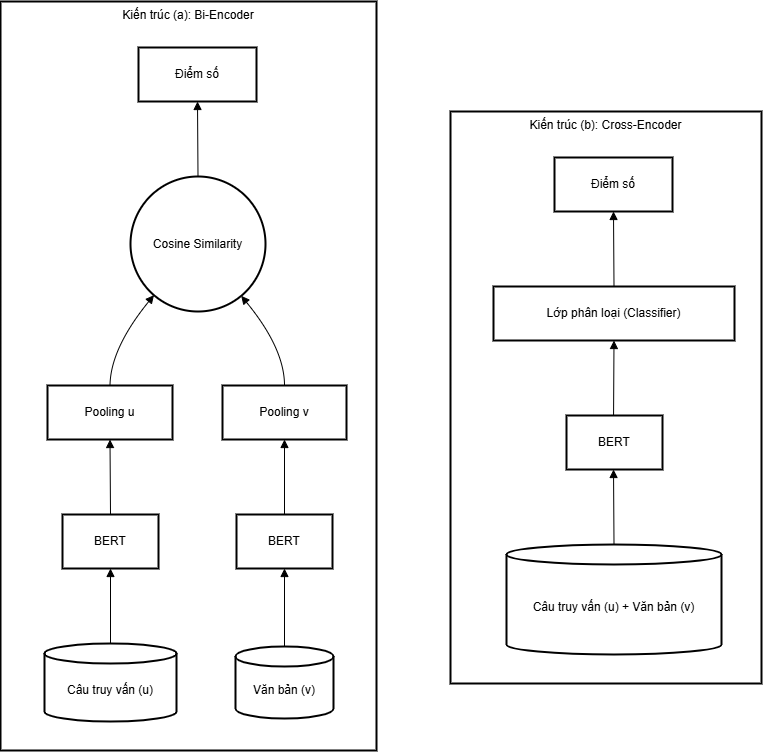
\includegraphics[width=0.8\textwidth]{images/so sanh.png}
    \caption{So sánh kiến trúc Bi-Encoder và Cross-Encoder}
    \label{fig:cross_bi_encoder}
\end{figure}

\subsection{Vai trò trong hệ thống truy xuất}
Trong bài toán truy xuất thông tin, luôn tồn tại sự đánh đổi giữa độ phủ (\textit{Recall}) và độ chính xác (\textit{Precision}). Các phương pháp truy xuất vector thường ưu tiên độ phủ để đảm bảo không bỏ sót thông tin, dẫn đến việc tập kết quả trả về có thể chứa nhiều tài liệu nhiễu hoặc không sát nghĩa.

Việc tích hợp Re-ranking đóng vai trò như một bộ lọc ngữ nghĩa cao cấp. Nhờ khả năng ``đọc hiểu'' sâu sắc mối quan hệ giữa câu hỏi và văn bản, Re-ranking giúp loại bỏ các kết quả dương tính giả (\textit{false positives}) và sắp xếp các tài liệu thực sự hữu ích lên vị trí đầu tiên. Các nghiên cứu thực nghiệm đã chứng minh rằng kiến trúc ``Truy xuất rồi Xếp hạng lại'' (\textit{Retrieve-then-Rerank}) mang lại hiệu suất vượt trội trên các bảng xếp hạng đánh giá truy xuất thông tin, đặc biệt trong các trường hợp truy vấn đòi hỏi khả năng suy luận phức tạp hoặc miền dữ liệu đặc thù \cite{thakur2021beir}.
% =========================================================
% SECTION 3.7: KNOWLEDGE BASE & VECTOR DB
% =========================================================
\section{Cơ sở tri thức và Cơ sở dữ liệu Vector}
\label{sec:kb_vector_db}

\subsection{Cơ sở tri thức (Knowledge Base)}
Trong các hệ thống trí tuệ nhân tạo hiện đại, Cơ sở tri thức (\textit{Knowledge Base - KB}) đóng vai trò là kho lưu trữ thông tin tập trung, chứa các dữ liệu, sự kiện và quy tắc mà hệ thống sử dụng để thực hiện việc suy luận hoặc ra quyết định. Đối với các bài toán xử lý ngôn ngữ tự nhiên, cơ sở tri thức thường tồn tại dưới dạng dữ liệu phi cấu trúc (\textit{unstructured data}) như văn bản, tài liệu PDF, hoặc biên bản cuộc họp \cite{russell2010artificial}.

Khác với các hệ thống cơ sở dữ liệu quan hệ truyền thống vốn yêu cầu dữ liệu phải được tổ chức chặt chẽ theo hàng và cột, cơ sở tri thức trong các ứng dụng AI chấp nhận sự đa dạng của dữ liệu tự nhiên. Tuy nhiên, thách thức lớn nhất là làm sao để truy xuất thông tin một cách hiệu quả dựa trên ý nghĩa nội dung thay vì chỉ so khớp từ khóa đơn thuần. Đây chính là tiền đề cho sự ra đời của các công nghệ lưu trữ vector.

\subsection{Cơ sở dữ liệu Vector (Vector Database)}
Để giải quyết bài toán quản lý và truy vấn cơ sở tri thức phi cấu trúc, Cơ sở dữ liệu Vector (\textit{Vector Database}) được sử dụng như một giải pháp chuyên dụng. Hệ thống này được thiết kế tối ưu để lưu trữ dữ liệu dưới dạng các vector nhiều chiều (\textit{embeddings}). Chức năng cốt lõi của nó là thực hiện \textbf{Tìm kiếm tương đồng (Similarity Search)}, tìm kiếm các vector trong không gian lưu trữ có khoảng cách hình học gần nhất với vector truy vấn thay vì tìm kiếm chính xác tuyệt đối \cite{han2023comprehensive}.

Các độ đo khoảng cách phổ biến bao gồm Khoảng cách Ơ-clít (\textit{Euclidean Distance}), Tích vô hướng (\textit{Dot Product}) và đặc biệt là Độ tương đồng Cosine (\textit{Cosine Similarity}) thường được dùng trong xử lý văn bản để đo độ tương đồng về ngữ nghĩa bất kể độ dài văn bản.

% --- MỤC MỚI BỔ SUNG: TEXT EMBEDDINGS ---
\subsection{Mô hình biểu diễn văn bản (Text Embeddings)}
Để lưu trữ văn bản vào cơ sở dữ liệu vector, cần có một cơ chế chuyển đổi ngôn ngữ tự nhiên thành các vector số học, gọi là quá trình \textit{Text Embedding}.

Khác với các phương pháp thống kê truyền thống (như TF-IDF hay Bag-of-Words) vốn không nắm bắt được ngữ nghĩa và gặp vấn đề thưa thớt dữ liệu, các mô hình Text Embedding hiện đại thường dựa trên kiến trúc Transformer (như BERT, RoBERTa) \cite{reimers2019sentence}. Các mô hình này, đặc biệt là các kiến trúc \textit{Dense Retrieval} (truy xuất dày đặc), có khả năng ánh xạ các câu văn có ý nghĩa tương đồng vào vị trí gần nhau trong không gian vector nhiều chiều, ngay cả khi chúng không chia sẻ từ vựng chung. Đây là thành phần then chốt quyết định độ chính xác của quá trình tìm kiếm ngữ nghĩa trong hệ thống RAG.

\subsection{Kỹ thuật chỉ mục (Indexing)}
Để đảm bảo tốc độ truy vấn trên các tập cơ sở tri thức lớn, việc so sánh vector truy vấn với toàn bộ dữ liệu (phương pháp vét cạn) là không khả thi. Do đó, các kỹ thuật chỉ mục \gls{ann} như \gls{hnsw} (\textit{Hierarchical Navigable Small World}) được áp dụng. \Gls{hnsw} tổ chức dữ liệu thành cấu trúc đồ thị phân cấp, cho phép thuật toán nhanh chóng định vị vùng không gian chứa thông tin liên quan với độ phức tạp tính toán thấp (thường là logarit), đảm bảo khả năng phản hồi thời gian thực \cite{malkov2018efficient}.


% =========================================================
% SECTION 3.9: LIMITATIONS & RAG SUPERIORITY
% =========================================================

\section{Cơ sở lý thuyết về RAG }
\label{sec:llm-limitations-rag}

% --- MỤC MỚI THÊM: ĐỊNH NGHĨA LLM ---
\subsection{Tổng quan về Mô hình Ngôn ngữ Lớn (LLM)}
\label{subsec:llm_overview}

Mô hình ngôn ngữ lớn (\textit{Large Language Model - LLM}) đại diện cho bước tiến quan trọng nhất trong lĩnh vực Xử lý ngôn ngữ tự nhiên (NLP) hiện đại. Về bản chất, đây là các mô hình học sâu (\textit{Deep Learning}) được xây dựng dựa trên kiến trúc Transformer, đặc trưng bởi cơ chế sự chú ý (\textit{Self-Attention}) giúp mô hình nắm bắt được các mối quan hệ ngữ nghĩa xa và phức tạp trong văn bản \cite{vaswani2017attention}.

Các mô hình này (như GPT-4, Gemini, Llama) được huấn luyện trên hàng tỷ tham số với lượng dữ liệu văn bản khổng lồ (thường là quy mô toàn bộ Internet) \cite{team2024gemini}. Cơ chế hoạt động cốt lõi của LLM là dự đoán từ tiếp theo (\textit{next-token prediction}) dựa trên xác suất thống kê từ chuỗi văn bản đầu vào. Chính nhờ quy mô dữ liệu và kiến trúc này, LLM sở hữu khả năng vượt trội trong việc hiểu ngữ cảnh, tóm tắt văn bản, dịch thuật và lập luận logic, tạo tiền đề cho các ứng dụng AI tạo sinh (\textit{Generative AI}).

% --- MỤC CŨ: HẠN CHẾ ---
\subsection{Hạn chế của LLM: Vấn đề ảo giác và Tri thức tĩnh}
Mặc dù sở hữu năng lực xử lý ngôn ngữ mạnh mẽ như đã đề cập, các mô hình LLM vẫn tồn tại những hạn chế cố hữu đã được cộng đồng nghiên cứu và doanh nghiệp ghi nhận. Vấn đề nghiêm trọng nhất là hiện tượng ``ảo giác'' (\textit{hallucinations}) - xu hướng của mô hình trong việc tạo ra các câu trả lời với văn phong tự tin, trôi chảy nhưng lại sai lệch hoàn toàn về mặt thực tế hoặc không liên quan đến truy vấn \cite{ji2023survey}.

Nguyên nhân chính của vấn đề này xuất phát từ bản chất ``học xác suất'' của mô hình: LLM không thực sự ``biết'' sự thật, mà chỉ dự đoán chuỗi từ ngữ hợp lý nhất. Thêm vào đó, LLM phụ thuộc hoàn toàn vào dữ liệu huấn luyện tĩnh (\textit{Static Knowledge}) \cite{team2024gemini}. Khi đối mặt với các câu hỏi đòi hỏi thông tin cập nhật mới nhất hoặc dữ liệu đặc thù của doanh nghiệp (như thông số sản phẩm, chính sách nội bộ), mô hình thường thất bại trong việc đưa ra câu trả lời chính xác do thiếu ngữ cảnh.

% --- GIẢI PHÁP RAG ---
\subsection{Giải pháp RAG: Neo giữ thông tin và Kiến trúc lai}
\label{subsec:rag_solution}

% --- PHẦN 1: GIỚI THIỆU & LỢI ÍCH ---
Kiến trúc \gls{rag} ra đời để giải quyết trực tiếp các hạn chế của LLM bằng cơ chế \textit{neo giữ} (\textit{grounding}) đầu ra của mô hình vào các nguồn tri thức bên ngoài tin cậy. Cách tiếp cận này mang lại hiệu quả vượt trội về độ chính xác. Các báo cáo từ khối doanh nghiệp chỉ ra rằng việc áp dụng RAG có thể nâng độ chính xác của các truy vấn nghiệp vụ lên trên 90\%, biến các mô hình ngôn ngữ tổng quát thành các trợ lý chuyên gia đáng tin cậy.

% --- PHẦN 2: ĐỊNH NGHĨA HÌNH THỨC ---
\subsubsection{Định nghĩa hình thức và Cơ chế hoạt động}
Về mặt bản chất kỹ thuật, theo định nghĩa gốc của Lewis và cộng sự \cite{lewis2020retrieval}, RAG là một kiến trúc lai (\textit{hybrid architecture}) kết hợp sức mạnh của hai loại bộ nhớ:
\begin{enumerate}
    \item \textbf{Bộ nhớ tham số (Parametric Memory):} Là các trọng số đã được huấn luyện trước của LLM, chứa khả năng ngôn ngữ và tri thức tổng quát.
    \item \textbf{Bộ nhớ phi tham số (Non-parametric Memory):} Là một chỉ mục vector chứa dữ liệu bên ngoài (biên bản cuộc họp, tài liệu), có thể cập nhật thời gian thực mà không cần huấn luyện lại mô hình \cite{lewis2020retrieval}.
\end{enumerate}

Dưới góc độ xác suất, với một truy vấn đầu vào $x$, RAG tính toán xác suất của câu trả lời $y$ bằng cách biên duyên hóa (\textit{marginalize}) qua các tài liệu $z$ được tìm thấy \cite{lewis2020retrieval}:
\begin{equation}
    p_{RAG}(y|x) \approx \sum_{z \in TopK(x)} p_\eta(z|x) \cdot p_\theta(y|x, z)
\end{equation}

Trong đó, hệ thống được cấu thành từ hai phân hệ cốt lõi hoạt động tuần tự:

\paragraph{1. Bộ truy xuất (The Retriever - $p_\eta$):} 
Chịu trách nhiệm ánh xạ câu hỏi $x$ và tài liệu $d$ vào cùng một không gian vector. Độ tương đồng được tính toán (thường bằng tích vô hướng hoặc Cosine) để tìm ra top-k tài liệu liên quan nhất, thường sử dụng kỹ thuật \textit{Dense Passage Retrieval} \cite{karpukhin2020dense}:
\begin{equation}
    score(x, d) = Encoder_Q(x)^T \cdot Encoder_D(d)
\end{equation}

\paragraph{2. Bộ tạo sinh (The Generator - $p_\theta$):} 
Là mô hình ngôn ngữ nhận đầu vào là sự kết hợp giữa truy vấn gốc và ngữ cảnh vừa tìm được ($Input = x \oplus z$). Nhờ cơ chế Attention và kỹ thuật Prompt Engineering \cite{liu2023pre}, mô hình sẽ sử dụng thông tin trong $z$ làm cơ sở dữ liệu để sinh ra câu trả lời $y$ chính xác và có thể kiểm chứng.

\subsection{Ứng dụng thực tiễn và Bảo mật dữ liệu}
Tầm quan trọng của RAG còn được thể hiện qua khả năng khai thác an toàn dữ liệu độc quyền (\textit{proprietary data}). 

Nhờ khả năng chuyển đổi LLM từ trạng thái chung chung sang trạng thái ``nhận thức ngữ cảnh'' (\textit{context-aware}), RAG hiện đã trở thành phương pháp tiếp cận tiêu chuẩn của ngành công nghiệp (\textit{industry-standard approach}). 

\begin{table}[h]
    \centering
    \caption{So sánh hiệu quả giữa LLM thuần túy và RAG trong doanh nghiệp}
    \label{tab:rag-vs-llm-business}
    \begin{tabular}{|p{4cm}|p{5cm}|p{5cm}|}
        \hline
        \textbf{Tiêu chí} & \textbf{LLM Thuần túy} & \textbf{RAG (Đồ án áp dụng)} \\
        \hline
        \textbf{Độ chính xác} & Dễ gặp ảo giác \cite{ji2023survey}, thông tin chung chung. & Cao ($>90\%$), được neo giữ bởi dữ liệu thực. \\
        \hline
        \textbf{Cập nhật kiến thức} & Bị giới hạn bởi thời điểm huấn luyện (Knowledge Cutoff) \cite{team2024gemini}. & Cập nhật tức thời theo thời gian thực (Real-time). \\
        \hline
        \textbf{Chi phí vận hành} & Tốn kém nếu phải Retrain liên tục. & Thấp, chỉ cần cập nhật Vector DB. \\
        \hline
        \textbf{Dữ liệu riêng tư} & Rủi ro lộ lọt nếu dùng để huấn luyện. & An toàn, dữ liệu nằm trong hệ thống kiểm soát nội bộ. \\
        \hline
    \end{tabular}
\end{table}

\section{Số liệu đánh giá}
\subsection{Các chỉ số đánh giá (Evaluation Metrics)}

Phần này trình bày các chỉ số đánh giá được sử dụng trong toàn bộ hệ thống, bao phủ từ mức tín hiệu (speech processing) đến mức suy luận ngữ nghĩa (RAG). Các chỉ số được thiết kế nhằm phản ánh đầy đủ các tiêu chí: độ chính xác, khả năng bảo toàn thông tin, và hiệu quả truy xuất.

\subsubsection{Diarization Metrics}

\textbf{Vai trò:}
Đánh giá chất lượng của mô-đun định danh người nói, là bước nền tảng ảnh hưởng trực tiếp đến toàn bộ pipeline phía sau.

\textbf{Diarization Error Rate (DER):}

DER là chỉ số tiêu chuẩn để đo lường mức độ sai lệch giữa kết quả diarization và ground truth theo thời gian.

\[
DER = \frac{Miss + FalseAlarm + Confusion}{Total\ Speech\ Time}
\]

Trong đó:
\begin{itemize}
    \item \textbf{Miss (Missed Speech):} phần speech không được phát hiện
    \item \textbf{False Alarm:} phần không phải speech nhưng bị phát hiện nhầm
    \item \textbf{Confusion:} phần speech được gán sai người nói
\end{itemize}

Trong phạm vi hệ thống, phân tích tập trung chủ yếu vào:
\begin{itemize}
    \item \textbf{Miss:} ảnh hưởng trực tiếp đến việc mất thông tin đầu vào cho ASR
    \item \textbf{Confusion:} ảnh hưởng đến tính đúng đắn của metadata speaker, từ đó tác động đến retrieval và QA
\end{itemize}

\textbf{Speaker Matching (Label Alignment):}

Do nhãn speaker trong hệ thống mang tính ký hiệu (arbitrary), cần thực hiện bước ánh xạ nhãn giữa kết quả dự đoán và ground truth trước khi tính DER.

Bài toán này được mô hình hóa như một bài toán gán tối ưu và được giải bằng thuật toán Hungarian, dựa trên ma trận nhầm lẫn (confusion matrix) ở mức frame.

\textbf{Phân tích lỗi:}
\begin{itemize}
    \item Label oscillation (dao động nhãn)
    \item Over-merging (gộp nhiều speaker)
    \item Over-splitting (tách một speaker thành nhiều nhãn)
\end{itemize}

Các phân tích này được sử dụng như công cụ chẩn đoán nhằm cải thiện pipeline, không phải là chỉ số định lượng độc lập.

\textbf{Speaker-Aware Coverage (SAC):}

SAC là chỉ số bổ sung nhằm đo lường khả năng bảo toàn nội dung gắn với đúng speaker.

\begin{itemize}
    \item \textbf{Coverage:} tỷ lệ các từ/cụm từ có nghĩa trong Ground Truth xuất hiện trong output
    \item \textbf{Speaker Correctness:} tỷ lệ các từ được gán đúng speaker
\end{itemize}

SAC giúp đánh giá tác động của lỗi diarization lên các bước downstream, đặc biệt là truy xuất và tổng hợp thông tin.

\subsubsection{Summarization Metrics}

\textbf{Vai trò:}
Đánh giá khả năng của hệ thống trong việc rút gọn dữ liệu hội thoại dài thành biểu diễn cô đọng, đồng thời vẫn giữ được thông tin quan trọng phục vụ truy xuất.

\begin{itemize}
    \item \textbf{Coverage:} 
    Tỷ lệ các điểm thông tin quan trọng được giữ lại trong bản tóm tắt. 
    Ngưỡng yêu cầu tối thiểu là 70\%.

    \item \textbf{Compression Ratio:} 
    Tỷ lệ giữa độ dài văn bản tóm tắt và văn bản gốc, được kiểm soát trong khoảng 20\%–40\%.

    \item \textbf{Faithfulness:} 
    Đảm bảo nội dung tóm tắt không chứa thông tin không xuất hiện trong ngữ cảnh đầu vào (không hallucination).
\end{itemize}

\subsubsection{Retrieval Metrics}

\textbf{Vai trò:}
Đánh giá khả năng của hệ thống trong việc truy xuất đúng và ưu tiên các đoạn hội thoại chứa thông tin quan trọng.

\begin{itemize}
    \item \textbf{Hit Rate@K:} 
    Tỷ lệ truy vấn mà đoạn chứa đáp án đúng xuất hiện trong Top-$K$ kết quả.

    \item \textbf{Mean Reciprocal Rank (MRR):}
    \[
    MRR = \frac{1}{Q} \sum_{i=1}^{Q} \frac{1}{rank_i}
    \]
    Đánh giá mức độ ưu tiên của các kết quả đúng trong danh sách truy xuất.

    \item \textbf{Context Relevance:}
    Đo lường mức độ liên quan của ngữ cảnh truy xuất so với truy vấn, phản ánh khả năng loại bỏ thông tin nhiễu trước khi đưa vào mô hình sinh.
\end{itemize}

\subsubsection{Metadata Impact}

\textbf{Vai trò:}
Đánh giá mức độ đóng góp của metadata (speaker, timestamp) đối với hiệu năng truy xuất và hỏi đáp.

\begin{itemize}
    \item So sánh HitRate@K và MRR giữa hai cấu hình:
    \begin{itemize}
        \item Có sử dụng metadata
        \item Không sử dụng metadata
    \end{itemize}
\end{itemize}

Kết quả so sánh cho phép xác định vai trò của thông tin speaker trong việc giảm nhiễu ngữ nghĩa và cải thiện độ chính xác của hệ thống.

\chapter{Thiết Kế \& Hiện Thực Hệ Thống}
% 1. Tổng quan (Chung)
% --- FILE: section/4.system/4.1_architecture_overview.tex ---

\section{Tổng quan kiến trúc hệ thống}
\label{sec:architecture_overview}

\subsection{Mô hình kiến trúc tổng thể}
Hệ thống được thiết kế theo mô hình đường ống (\textit{Pipeline Architecture}), chia thành các mô-đun xử lý tuần tự nhằm giải quyết bài toán truy xuất thông tin từ dữ liệu âm thanh hội họp phức tạp. Mục tiêu thiết kế là đảm bảo khả năng xử lý các cuộc họp kéo dài, đa người nói và cung cấp câu trả lời có độ chính xác cao dựa trên ngữ cảnh thực tế.

Kiến trúc tổng thể của hệ thống bao gồm hai mô-đun chính hoạt động liên kết chặt chẽ:
\begin{enumerate}
    \item \textbf{Mô-đun Xử lý tiếng nói (Speech Processing Module):} Chịu trách nhiệm chuyển đổi dữ liệu âm thanh thô thành văn bản có cấu trúc, bao gồm việc định danh người nói (\textit{Speaker Diarization}) và nhận dạng nội dung (\textit{ASR}).
    \item \textbf{Mô-đun Truy xuất và Tạo sinh tri thức (RAG Module):} Thực hiện việc lưu trữ, đánh chỉ mục vector và sử dụng mô hình ngôn ngữ lớn (\textit{LLM}) để trả lời câu hỏi dựa trên văn bản đã được trích xuất.
\end{enumerate}

Sự tách biệt giữa hai mô-đun này giúp hệ thống đạt được tính độc lập cao, dễ dàng nâng cấp từng thành phần (ví dụ: thay đổi model ASR hoặc model Embedding) mà không ảnh hưởng đến toàn bộ cấu trúc.

% \begin{figure}[h]
%     \centering
%     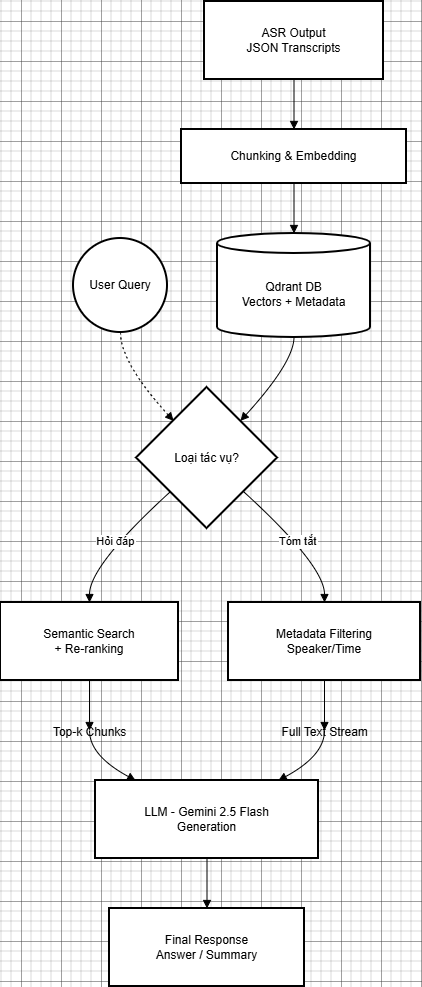
\includegraphics[width=0.9\textwidth]{images/RAG_pipline.png}
%     \caption{Sơ đồ kiến trúc tổng thể của hệ thống hỗ trợ cuộc họp thông minh}
%     \label{fig:system_overview}
% \end{figure}

\subsection{Luồng dữ liệu trong hệ thống}
Dữ liệu trong hệ thống được luân chuyển và biến đổi qua 4 giai đoạn chính, đảm bảo tính vẹn toàn từ tín hiệu âm thanh đến câu trả lời cuối cùng:

\begin{itemize}
    \item \textbf{Giai đoạn 1: Thu thập và Tiền xử lý (Ingestion).} Đầu vào là các bản ghi âm cuộc họp (Meeting Recordings). Các bản ghi này thường chứa tạp âm và có nhiều người tham gia. Hệ thống thực hiện chuẩn hóa âm thanh để tối ưu cho bước nhận dạng.
    
    \item \textbf{Giai đoạn 2: Chuyển đổi cấu trúc (Transcribing \& Diarization).} Phân hệ ASR xử lý tín hiệu âm thanh để tách biệt các đoạn thoại của từng diễn giả và chuyển đổi thành văn bản. Kết quả đầu ra không chỉ là chuỗi ký tự đơn thuần mà là dữ liệu bán cấu trúc (\textit{Semi-structured Data}) chứa thông tin siêu dữ liệu (\textit{Metadata}) quan trọng: định danh người nói (\textit{Speaker ID}) và mốc thời gian (\textit{Timestamp}).
    
    \item \textbf{Giai đoạn 3: Đánh chỉ mục tri thức (Indexing).} Dữ liệu văn bản kèm metadata được phân hệ RAG tiếp nhận. Tại đây, kỹ thuật \textit{Chunking} thông minh được áp dụng để chia nhỏ hội thoại nhưng vẫn giữ nguyên ngữ cảnh. Các đoạn văn bản này sau đó được mã hóa thành vector (\textit{Embeddings}) và lưu trữ trong Cơ sở dữ liệu Vector để phục vụ truy vấn.
    
    \item \textbf{Giai đoạn 4: Truy xuất và Tổng hợp (Retrieval \& Generation).} Khi người dùng đặt câu hỏi (ví dụ: ``Ai đề xuất phương án A?''), hệ thống thực hiện tìm kiếm ngữ nghĩa (\textit{Semantic Search}) kết hợp xếp hạng lại (\textit{Re-ranking}). Các đoạn hội thoại liên quan nhất được trích xuất và đưa vào LLM để sinh câu trả lời, kèm theo dẫn chứng cụ thể về thời gian và người nói.
\end{itemize}

\subsection{Các nguyên lý thiết kế cốt lõi}
Dựa trên đặc thù của bài toán xử lý biên bản cuộc họp, hệ thống tuân thủ các nguyên tắc thiết kế sau:

\begin{enumerate}
    \item \textbf{Tính truy vết (Traceability):} Mọi thông tin do LLM sinh ra đều phải được neo giữ (\textit{grounded}) vào dữ liệu gốc. Hệ thống được thiết kế để luôn trả về nguồn gốc của thông tin (trích đoạn âm thanh tại giây thứ bao nhiêu, do ai nói) để người dùng có thể đối chiếu, đặc biệt quan trọng trong các lĩnh vực pháp lý và y tế.
    \item \textbf{Khả năng chống nhiễu (Robustness):} Nhận thức được việc transcript từ ASR có thể chứa sai sót nhận dạng, cơ chế tìm kiếm Vector được tối ưu hóa để nắm bắt ý nghĩa ngữ nghĩa tổng quát thay vì chỉ so khớp từ khóa chính xác, giúp hệ thống vẫn tìm được thông tin đúng ngay cả khi văn bản có lỗi sai chính tả nhỏ.
    \item \textbf{Xử lý ngữ cảnh dài (Long-context Handling):} Với các cuộc họp kéo dài hàng giờ, hệ thống sử dụng chiến lược cửa sổ trượt (\textit{sliding window}) và bộ nhớ đệm hội thoại để đảm bảo LLM không bị mất ngữ cảnh khi xử lý các câu hỏi phức tạp hoặc các yêu cầu tóm tắt đa tầng (\textit{multi-level summarization}).
\end{enumerate}
\section{Mô hình Xử lý tiếng nói (Speech Processing Module)}
Mô hình Xử lý tiếng nói đóng vai trò là lớp chuyển đổi trung gian giữa tín hiệu âm thanh thô và biểu diễn văn bản có cấu trúc, làm cơ sở cho toàn bộ các bước truy xuất tri thức phía sau. Mô hình này được thiết kế để bảo toàn thông tin ngữ cảnh hội thoại, đặc biệt là định danh người nói và mốc thời gian.

Vì vậy, kết quả của mô hình không đơn thuần là transcript, mà là một tập các phân đoạn hội thoại được thêm dữ liệu ngoài hội thoại, đóng vai trò là dữ liệu cơ sở cho quá trình đánh chỉ mục và truy xuất sau này.

Mô hình được phân thành 2 phần chính:
\begin{itemize}
    \item Định danh người nói (Speaker Diarization).
    \item Nhận dạng tiếng nói tự động (Automatic Speech Recognition - ASR). 
\end{itemize}

Hai phần này hoạt động tuần tự, kết quả của Diarization quyết định các phân đoạn được đưa vào ASR, đồng thời cung cấp thông tin người nói để gán nhãn cho văn bản được sinh ra. Việc hoạt động tuần tự là cần thiết, vì các mô hình ASR tốn kém chi phí vận hành, xử lý dữ liệu qua Diarization giúp tách biệt lời nói rõ ràng giữa những diễn giả, từ đó hạn chế trộn lẫn ngữ cảnh giữa các đoạn hội thoại và cũng giúp khử nhiễu, giữ cho mô hình ASR hoạt động ổn định hơn so với bản ghi liên tục.

\subsection{Định danh người nói}
Ở bước đầu tiên, tín hiệu âm thanh đầu vào được xử lý bằng mô-đun phát hiện hoạt động giọng nói (VAD) nhằm xác định các khoảng thời gian có lời nói. Các đoạn lời nói sau đó được phân loại thành hai nhóm dựa trên độ dài: các đoạn đủ dài để trích xuất embedding ổn định và các đoạn ngắn không đạt ngưỡng tối thiểu.

Việc tách riêng các đoạn ngắn ngay từ đầu nhằm tránh việc đưa các embedding kém ổn định vào quá trình phân cụm chính, vốn có thể dẫn tới các lỗi gộp hoặc tách nhãn không mong muốn.

\textbf{Phân cụm thô với Embedding cỡ lớn}:
Các đoạn giọng nói đủ dài được sử dụng để trích xuất speaker embedding bằng các mô hình chuyên dụng (như ECAPA-TDNN hoặc TitaNet-large). Các mô hình này có tính phân biệt cao và phù hợp cho việc xây dựng cấu trúc phân cụm ổn định trong không gian đặc trưng.

Tập embedding thu được được đưa vào mô-đun phân cụm nhằm ước lượng số lượng người nói và gán nhãn sơ bộ cho các đoạn giọng nói dài. Kết quả của pha này được xem là các cụm thô (coarse clusters), đóng vai trò nền tảng cho các bước xử lý tiếp theo.

\textbf{Khởi tạo đại diện cụm (Cluster pivots)}: Sau khi hoàn tất pha phân cụm thô, mỗi cụm người nói được đại diện bởi một tập con các đoạn giọng nói tiêu biểu. Các đoạn này được sử dụng để xây dựng các vector đại diện (pivot embeddings) cho từng cụm, nhằm tạo cầu nối giữa không gian embedding cỡ lớn và không gian embedding ở pha tiếp theo.

Các pivot này cho phép chuyển thông tin về cấu trúc người nói đã được ước lượng sang không gian embedding khác, đồng thời giảm thiểu ảnh hưởng của nhiễu do các đoạn giọng nói ngắn gây ra.

\textbf{Gán nhãn bổ sung}: Các đoạn giọng nói ngắn bị loại khỏi pha phân cụm ban đầu được xử lý riêng. Các đoạn này được trích xuất embedding bằng một mô hình biểu diễn có khả năng xử lý hiệu quả các phân đoạn ngắn và giàu ngữ cảnh cục bộ.

Embedding của các đoạn ngắn được so sánh với các vector đại diện của từng cụm thu được từ gom cụm thô. Nhãn người nói được gán dựa trên độ tương đồng cao nhất, đảm bảo mọi đoạn giọng nói đều được gán nhãn mà không làm thay đổi cấu trúc phân cụm đã được xác định trước đó.

Cuối cùng, các đoạn giọng nói được hợp nhất theo trật tự thời gian để tạo ra kết quả diarization hoàn chỉnh. Pipeline đảm bảo rằng tất cả các đoạn lời nói, bao gồm cả các đoạn ngắn, đều được gán nhãn người nói tương ứng, đồng thời giữ nguyên cấu trúc phân cụm ổn định từ pha đầu tiên.

Thiết kế hai bước gán nhãn tách biệt rõ ràng nhằm hạn chế ảnh hưởng lỗi từ các đoạn ngắn của những embeddings cỡ lớn đến cấu trúc phân cụm, và tối ưu ưu điểm của hai loại mô hình embeddings hiện đại.

\subsection{Mô hình Tự động Nhận diện Giọng nói}
ASR trong hệ thống không chỉ đảm nhiệm chức năng chuyển đổi tín hiệu âm thanh sang văn bản, mà còn đóng vai trò chuẩn hóa cấu trúc hội thoại để phục vụ các bước xử lý ngữ nghĩa và truy xuất tri thức phía sau.

\textbf{Gán nhãn người nói cho văn bản ASR}
Sau khi hoàn tất quá trình Diarization, mỗi phân đoạn giọng nói được gắn nhãn và mốc thời gian. Mỗi phân đoạn không được xem là độc lập hoàn toàn trong quá trình nhận dạng tiếng nói. Trong thực tế, các phân đoạn này thường bị phân mảnh do hiện tượng cắt lời, dao động nhãn (oscillation) hoặc tách đoạn quá mức, dẫn đến độ dài ngữ cảnh không tối ưu cho ASR.

\textbf{Xử lý phân mảnh trước ASR}
Kết quả phân tích Diarization cho thấy một số lỗi còn tồn động như oscillation, merge và split, đặc biệt ở các đoạn hội thoại ngắn liên tiếp. Điều này làm suy giảm hiệu quả trong suy đoán ngữ cảnh của ASR nếu áp dụng trực tiếp lên từng đoạn riêng biệt. Vì vậy, mô hình thực hiện ASR theo từng cụm phân đoạn (segment grouping), trong đó các đoạn gần nhau về mặt thời gian được gom lại thành các đơn vị lớn hơn.

Việc gom nhóm phân đoạn được điều khiển bởi một ngưỡng độ dài tối thiểu, nhằm đảm bảo mỗi đơn vị đầu vào cho ASR chứa đủ thông tin ngữ âm và ngữ cảnh để mô hình hoạt động ổn định. Cách tiếp cận này giúp giảm thiểu các lỗi nhận dạng do ngữ cảnh quá ngắn, đồng thời hạn chế việc phá vỡ cấu trúc hội thoại gốc.

Để cân bằng giữa việc bảo toàn ranh giới hội thoại và yêu cầu về độ dài ngữ cảnh, hệ thống áp dụng chiến lược soft-padding sliding window. Cụ thể, mỗi cụm phân đoạn được mở rộng thêm một khoảng ngữ cảnh ngắn ở hai phía (trước và sau), với các đoạn đệm này không được xem là trung tâm nhận dạng nhưng cung cấp thêm thông tin ngữ cảnh cho mô hình ASR. Sau khi hoàn tất nhận dạng, chỉ phần văn bản tương ứng với vùng trung tâm của cửa sổ được giữ lại, trong khi phần đệm được loại bỏ nhằm tránh trùng lặp nội dung.

\textbf{Hiệu chỉnh cấu trúc hội thoại dựa trên mô hình ngôn ngữ lớn}
Mặc dù chiến lược gom cụm phân đoạn và soft-padding sliding window giúp ổn định đầu vào cho ASR, đầu ra văn bản thu được vẫn có thể chưa phản ánh chính xác cấu trúc hội thoại thực tế. Nguyên nhân là các ranh giới phân đoạn được xác định ở mức tín hiệu âm thanh không luôn tương thích với ranh giới cú pháp và ngữ nghĩa ở mức văn bản, đặc biệt trong các tình huống hội thoại nhanh, cắt lời hoặc phản
hồi ngắn. 

Do đó, hệ thống áp dụng một bước hậu xử lý dựa trên mô hình ngôn ngữ lớn (LLM) nhằm hiệu chỉnh ranh giới giữa các đoạn hội thoại dựa trên cấu trúc câu và ngữ nghĩa tổng thể của transcript. Mô hình ngôn ngữ trong bước này không sinh thêm nội dung mới, mà chỉ thực hiện việc gộp hoặc tách các đoạn văn bản để đảm bảo tính nhất quán về mặt hội thoại trước khi chuyển sang giai đoạn đánh chỉ mục và truy xuất tri thức.

Bước hiệu chỉnh này được đặt sau phân hệ ASR và được xem là cần thiết để giảm thiểu tác động của hiện tượng phân mảnh phân đoạn và các lỗi tồn động từ quá trình diarization, mặc dù hiện chưa có thước đo định lượng trực tiếp cho bước xử lý này. 


% --- FILE: 4.3_rag_pipeline/4.3.0_intro.tex ---

\section{Mô hình Truy xuất và Tạo sinh tri thức (RAG Module)}
\label{sec:rag_pipeline}

Tiếp nối kết quả từ quá trình chuyển đổi giọng nói sang văn bản, mô-đun \gls{rag} đóng vai trò trung tâm trong việc tổ chức, khai thác và tổng hợp tri thức từ dữ liệu hội thoại. Dựa trên đầu vào là các tệp JSON có cấu trúc (chứa thông tin người nói, thời gian và nội dung) từ mô-đun ASR, mô-đun này được thiết kế để thực hiện hai nhóm chức năng cốt lõi:\textit{Truy xuất thông tin theo ngữ cảnh} (phục vụ hỏi đáp) và \textit{Tổng hợp nội dung đa tầng}(phục vụ tóm tắt).

Để hiện thực hóa các chức năng trên, mô-đun vận hành theo một quy trình xử lý khép kín gồm bốn giai đoạn kỹ thuật chính:

\begin{enumerate}
    \item \textbf{Indexing (Đánh chỉ mục):} Mã hóa văn bản thành vector và lưu trữ vào cơ sở dữ liệu chuyên dụng, kèm theo siêu dữ liệu để phục vụ lọc thông tin.
    \item \textbf{Retrieval (Truy xuất):} Tìm kiếm các đoạn hội thoại liên quan nhất đến câu hỏi dựa trên ngữ nghĩa (Semantic Search) và xếp hạng lại (Re-ranking) để loại bỏ nhiễu.
    \item \textbf{Generation (Tạo sinh):} Tích hợp \gls{llm} để sinh câu trả lời tự nhiên hoặc bản tóm tắt dựa trên ngữ cảnh đã trích xuất.
    \item \textbf{Summarization (Tổng hợp):} Áp dụng các kỹ thuật xử lý ngữ cảnh dài để tóm tắt toàn bộ cuộc họp hoặc tóm tắt theo từng đối tượng người nói cụ thể.
\end{enumerate}



\begin{figure}[H]
    \centering
    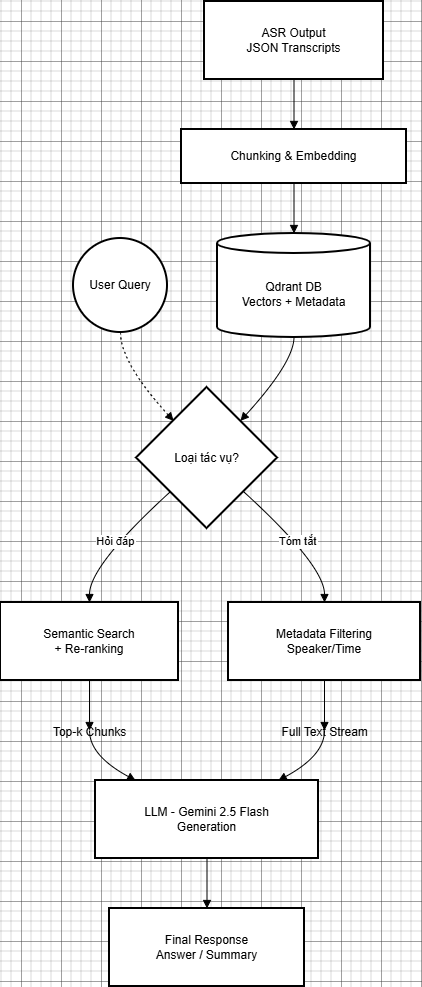
\includegraphics[width=0.6\textwidth]{images/RAG_pipline.png}
    \caption{Sơ đồ luồng xử lý dữ liệu tích hợp chức năng Tóm tắt trong mô-đun RAG}
    \label{fig:rag_detailed_flow}
\end{figure}
\clearpage
\subsection{Xây dựng và Đánh chỉ mục dữ liệu (Indexing)}
\label{subsec:indexing}

Giai đoạn đầu tiên của đường ống RAG là chuyển đổi dữ liệu hội thoại thô thành cấu trúc có thể tìm kiếm được. Quá trình này không chỉ đơn thuần là lưu trữ văn bản mà còn bao gồm việc làm sạch dữ liệu, mã hóa ngữ nghĩa (Vectorization) và thiết lập cơ sở dữ liệu vector tối ưu.

\subsubsection{Tiền xử lý và Chuẩn hóa dữ liệu đầu vào}
Hệ thống tiếp nhận đầu vào là các tệp JSON được sinh ra từ mô-đun ASR. Do đặc thù của dữ liệu hội thoại tự nhiên, thông tin đầu vào thường gặp các vấn đề như thiếu nhãn người nói hoặc định dạng không đồng nhất. Để đảm bảo tính toàn vẹn dữ liệu, quy trình chuẩn hóa (\textit{Data Sanitization}) được áp dụng trong phương thức \texttt{\_load\_memory\_kb} với các tiêu chí sau:

\begin{itemize}
    \item \textbf{Định danh lượt lời:} Mỗi lượt lời (utterance) được gán một định danh duy nhất (\texttt{utt\_id}) phục vụ truy vết.
    \item \textbf{Xử lý dữ liệu khuyết thiếu:} Hệ thống kiểm tra các trường bắt buộc (\texttt{speaker}, \texttt{text}). Cơ chế an toàn (\textit{Fail-safe}) sẽ gán giá trị mặc định (ví dụ: "Unknown Speaker") nếu dữ liệu bị thiếu nhằm tránh lỗi thực thi.
    \item \textbf{Tổng hợp toàn văn:} Song song với xử lý từng câu, hệ thống ghép nối nội dung thành chuỗi văn bản liền mạch (\texttt{full\_text}) phục vụ riêng cho tác vụ tóm tắt.
\end{itemize}

\begin{lstlisting}[language=Python, caption={Logic tiền xử lý dữ liệu hội thoại}, label={lst:preprocessing_logic}]
    def _load_memory_kb(self):
        # ... (Code for file reading omitted)
        for i, utt in enumerate(data):
            utt_id = f"utt_{i}"
            
            # Gan gia tri mac dinh neu thieu (Fail-safe mechanism)
            speaker = utt.get('speaker', 'Unknown Speaker')
            text = utt.get('text', '')
            
            # Luu tru metadata
            kb["utterances"][utt_id] = {
                'speaker': speaker,
                'text': text,
                'start': utt.get('start', 0)
            }
            full_text_list.append(f"{speaker}: {text}")
\end{lstlisting}

\subsubsection{Cấu hình Cơ sở dữ liệu Vector (Qdrant)}
Sau khi dữ liệu được làm sạch, hệ thống sử dụng \textit{Qdrant} để lưu trữ và đánh chỉ mục. Quá trình khởi tạo bao gồm thiết lập thuật toán HNSW và lựa chọn mô hình Embedding phù hợp.

\paragraph{Cấu hình Index (HNSW Configuration):}
Hệ thống sử dụng thuật toán HNSW để tối ưu hóa tốc độ tìm kiếm. Các tham số cấu hình trong lớp \texttt{HnswConfigDiff} được thiết lập dựa trên khuyến nghị thực nghiệm cho dữ liệu văn bản:
\begin{itemize}
    \item \textbf{Độ đo khoảng cách:} Sử dụng \texttt{Distance.COSINE} để đo độ tương đồng ngữ nghĩa.
    \item \textbf{Tham số $m=16$:} Số lượng liên kết tối đa cho mỗi node, giúp cân bằng giữa tốc độ truy vấn và bộ nhớ.
    \item \textbf{Tham số $ef\_construct=100$:} Độ sâu tìm kiếm khi xây dựng chỉ mục, đảm bảo độ chính xác cao (Recall) ngay từ đầu.
\end{itemize}

\paragraph{Mã hóa và Lưu trữ (Vectorization \& Upsert):}
Dựa trên lý thuyết về Text Embeddings, hệ thống sử dụng mô hình \texttt{BAAI/bge-m3} để chuyển đổi văn bản thành vector. Điểm đặc biệt trong kiến trúc lưu trữ là cơ chế \textit{Payload}:
\begin{itemize}
    \item \textbf{Vector:} Chỉ chứa thông tin ngữ nghĩa (\texttt{utt['text']}).
    \item \textbf{Payload (Siêu dữ liệu):} Lưu trữ bản gốc (\texttt{text\_original}), ID và người nói. Điều này cho phép hệ thống truy xuất ngược lại nội dung gốc ngay lập tức mà không cần tra cứu bảng dữ liệu thô bên ngoài.
\end{itemize}

\begin{lstlisting}[language=Python, caption={Quy trình khởi tạo Collection và nạp dữ liệu}, label={lst:db_build_logic}]
    # 1. Tao Collection voi cau hinh HNSW
    self.client.create_collection(
        collection_name=self.collection_name,
        vectors_config=VectorParams(size=EMBEDDING_DIM, distance=Distance.COSINE),
        hnsw_config=HnswConfigDiff(m=16, ef_construct=100)
    )
    
    # 2. Vector hoa va chuan bi Payload
    embeddings = embed_model.encode(docs, show_progress_bar=True)
    
    points = [
        PointStruct(
            id=ids[i], 
            vector=embeddings[i].tolist(), 
            payload={
                "text_original": utt['text'],
                "doc_id": uid,
                "speaker": utt['speaker']
            }
        ) 
        for i in range(len(ids))
    ]
    
    # 3. Batch Upsert (Nap du lieu theo lo)
    self.client.upsert(self.collection_name, points[i:i+batch_size])
\end{lstlisting}
    \subsection{Quy trình Truy xuất đa tầng (Multi-stage Retrieval)}
    \label{subsec:retrieval}
    
    % --- 1. PHẦN THIẾT KẾ (DESIGN) ---
    \subsubsection{Chiến lược thiết kế}
    Quy trình truy xuất được xây dựng theo kiến trúc đường ống hai giai đoạn (\textit{Retrieve-then-Rerank}). Chiến lược này nhằm giải quyết bài toán cân bằng giữa hiệu năng và độ chính xác:
    \begin{itemize}
        \item \textbf{Giai đoạn Truy xuất (Retrieval):} Sử dụng kiến trúc Bi-Encoder để tìm kiếm nhanh trong không gian vector, chấp nhận độ chính xác tương đối để đảm bảo không bỏ sót thông tin (\textit{High Recall}).
        \item \textbf{Giai đoạn Tái xếp hạng (Re-ranking):} Sử dụng kiến trúc Cross-Encoder để đánh giá sâu ngữ nghĩa từng cặp câu, loại bỏ nhiễu để đạt độ chính xác cao nhất (\textit{High Precision}).
    \end{itemize}
    \begin{figure}[H]
    \centering
    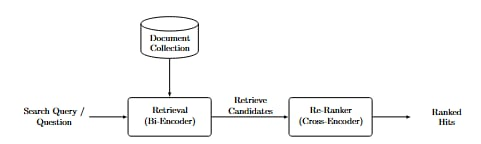
\includegraphics[width=1\textwidth]{images/retrieval.jpg}
    \caption{Sơ đồ quy trình truy xuất hai giai đoạn (Retrieval \& Re-ranking)}
    
\end{figure}
   
    
    % --- 2. PHẦN HIỆN THỰC (IMPLEMENTATION) ---
    \subsubsection{Chi tiết hiện thực kỹ thuật}
    Hệ thống được hiện thực hóa bằng thư viện \texttt{sentence-transformers} và \texttt{qdrant-client}, trải qua 4 bước xử lý tuần tự:
    
    \paragraph{Bước 1: Tìm kiếm Vector (Candidate Generation):}
    Mục tiêu là thu hẹp không gian tìm kiếm từ toàn bộ cơ sở dữ liệu xuống một tập ứng viên nhỏ.
    \begin{itemize}
        \item \textbf{Mã hóa:} Câu truy vấn được vector hóa và chuẩn hóa (\texttt{normalize\_embeddings=True}) để tương thích với độ đo Cosine.
        \item \textbf{Truy vấn Qdrant:} Hệ thống thực hiện \texttt{query\_points} với tham số giới hạn \texttt{limit=30}. Ngưỡng 30 này đóng vai trò là "Bộ lọc thô", đủ rộng để bao quát các ngữ cảnh tiềm năng.
        \item \textbf{Payload:} Dữ liệu trả về bao gồm cả văn bản gốc (\texttt{text\_original}) để phục vụ bước tiếp theo.
    \end{itemize}
    \begin{lstlisting}[language=Python,  label={lst:retrieval_logic}]
            query_vec = embed_model.encode([query], normalize_embeddings=True)[0].tolist()
            resp = self.client.query_points(
                    collection_name=self.collection_name,
                    query=query_vec,                 
                    # query_filter=query_filter,     
                    limit=30,
                    with_payload=True
                )
    
            hits = resp.points or []
            
            
            if not hits: return []
    \end{lstlisting}
    
    \paragraph{Bước 2: Đánh giá ngữ nghĩa chéo (Cross-Encoder Scoring):}
    Đây là bước tinh lọc quan trọng nhất. Hệ thống sử dụng mô hình \texttt{BAAI/bge-reranker-large} — một mô hình SOTA (State-of-the-art) về khả năng rerank đa ngôn ngữ.
    \begin{itemize}
        \item Hệ thống ghép cặp \texttt{(Câu hỏi, Đoạn văn bản)} từ 30 ứng viên ở Bước 1.
        \item Danh sách các cặp \texttt{[Query, Document]} này sau đó được đưa vào mô hình để thực hiện dự đoán song song (\texttt{prediction}), tạo ra điểm số tương đồng ngữ nghĩa chính xác cho từng ứng viên.
    \end{itemize}
    \begin{lstlisting}[language=Python,  label={lst:retrieval_logic}]
     # 2. Rerank
            pairs = []
            for hit in hits:
                if hit.payload:
                    pairs.append([query, hit.payload.get('text_original', '')])
            
            if not pairs: return []
    
            scores = rerank_model.predict(pairs) # type: ignore
    \end{lstlisting}
    \paragraph{Bước 3: Chọn lọc kết quả (Final Selection):}
    Dựa trên điểm số mới từ Cross-Encoder, danh sách được sắp xếp lại (\texttt{sorted}) theo thứ tự giảm dần.
    \begin{itemize}
        \item Hệ thống thực hiện cắt ngưỡng lấy \textbf{Top-5} kết quả tốt nhất (\texttt{[:5]}).
        \item \textbf{Ý nghĩa:} Con số 5 được lựa chọn thực nghiệm nhằm tối ưu hóa bộ nhớ đệm (Context Window) của LLM, đảm bảo mô hình chỉ nhận được những thông tin tinh túy nhất, giảm thiểu hiện tượng ảo giác do nhiễu thông tin.
    \end{itemize}
    \begin{lstlisting}[language=Python,  label={lst:retrieval_logic}]
     # Top 5
            ranked_hits = sorted(zip(scores, hits), key=lambda x: x[0], reverse=True)[:5]
    \end{lstlisting}
    \paragraph{Bước 4: Mở rộng ngữ cảnh (Context Augmentation):}
    Một thách thức đặc thù của dữ liệu hội thoại là tính liên kết ngữ nghĩa giữa các lượt lời. Một câu nói đơn lẻ (ví dụ: \textit{"Tôi đồng ý với ý kiến đó"}) sẽ trở nên vô nghĩa nếu thiếu câu nói trước đó. Để giải quyết vấn đề này, hệ thống áp dụng kỹ thuật \textbf{Cửa sổ trượt (Sliding Window)} để mở rộng ngữ cảnh xung quanh kết quả tìm kiếm.
    
    Dựa trên chỉ số (\textit{index}) của đoạn hội thoại tìm được trong chuỗi thời gian gốc, hệ thống thực hiện truy xuất thêm các đoạn lân cận:
    \begin{itemize}
        \item \textbf{Cơ chế:} Với mỗi kết quả $h_i$ tại vị trí $k$, hệ thống sẽ lấy thêm đoạn $k-1$ (lượt lời trước đó) và $k+1$ (lượt lời sau đó).
        \item \textbf{Mục đích:} Việc lấy thêm đoạn $k-1$ giúp giải quyết các tham chiếu đại từ (như "đó", "anh ấy"), trong khi đoạn $k+1$ cung cấp phản hồi ngay lập tức.
        \item \textbf{Hợp nhất \& Khử trùng:} Hệ thống sử dụng một tập hợp \texttt{processed\_ids} để đảm bảo các đoạn hội thoại không bị lặp lại nếu các kết quả tìm kiếm nằm quá gần nhau.
    \end{itemize}
    \begin{lstlisting}[language=Python,  label={lst:retrieval_logic}]
    # 3. Context Augmentation 
            final_chunks = []
            processed_ids = set()
            
            # Map ID to index 
            id_to_index = {uid: i for i, uid in enumerate(self.kb_memory["utterance_order"])}
            
            for score, hit in ranked_hits:
                if not hit.payload: continue
                doc_id = hit.payload.get('doc_id')
                if not doc_id or doc_id in processed_ids: continue
                
                idx = id_to_index.get(doc_id)
                if idx is None: continue
                
                # Window [idx-1, idx+1]
                start = max(0, idx - 1)
                end = min(len(self.kb_memory["utterance_order"]), idx + 2)
                
                chunk_text = []
                for i in range(start, end):
                    uid = self.kb_memory["utterance_order"][i]
                    processed_ids.add(uid)
                    u = self.kb_memory["utterances"][uid]
                    chunk_text.append(f"[{u['start']}] {u['speaker']}: {u['text']}")
                
                final_chunks.append("\n".join(chunk_text))
                
            return final_chunks
    \end{lstlisting}
% --- FILE: 4.3_rag_pipeline/4.3.3_generation.tex ---

\subsection{Tích hợp Mô hình ngôn ngữ và Tạo sinh (Generation)}
\label{subsec:generation}

Cơ chế tạo sinh đóng vai trò quan trọng trong việc sản xuất kết quả cuối cùng bằng cách tích hợp thông tin được truy xuất với truy vấn đầu vào. Sau khi thành phần truy xuất lấy kiến thức liên quan từ các nguồn bên ngoài, bộ tạo sinh tổng hợp thông tin này thành các phản hồi mạch lạc và phù hợp với ngữ cảnh. Mô hình Ngôn ngữ Lớn (LLM) đóng vai trò là xương sống của bộ tạo sinh, đảm bảo văn bản được tạo ra trôi chảy, chính xác và phù hợp với truy vấn gốc.

% --- SỬA ĐỔI: Nâng paragraph lên thành subsubsection ---
\subsubsection{Lựa chọn Mô hình (Model Selection)}
Hệ thống sử dụng \textit{Google Gemini 2.5 Flash} làm mô hình nền tảng (\textit{Foundation Model}). Quyết định này dựa trên báo cáo kỹ thuật của Google \cite{team2024gemini}, trong đó nhấn mạnh ưu thế vượt trội của kiến trúc này về khả năng xử lý \textit{Cửa sổ ngữ cảnh siêu lớn (Long Context Window)}. Khả năng này cho phép hệ thống nạp đồng thời nhiều đoạn hội thoại dài vào bộ nhớ đệm mà không làm mất mát thông tin, khắc phục hạn chế về độ dài đầu vào của các mô hình Transformer truyền thống.

\subsubsection{Kỹ thuật Viết lại câu hỏi (Query Rewriting)}
Một thách thức lớn trong hội thoại tự nhiên là sự xuất hiện của các đại từ thay thế (như "nó", "ông ấy") hoặc các câu hỏi tỉnh lược. Để giải quyết vấn đề này, hệ thống áp dụng cơ chế viết lại câu hỏi trước khi thực hiện truy xuất nhằm đảm bảo tính đầy đủ của ngữ nghĩa. Cụ thể, hệ thống sẽ trích xuất lịch sử ba lượt hội thoại gần nhất và gửi đến mô hình ngôn ngữ lớn một yêu cầu chuyển đổi. Mô hình sẽ phân tích ngữ cảnh và thay thế các đại từ hoặc thành phần bị lược bỏ bằng các danh từ cụ thể đã xuất hiện trước đó. Câu hỏi sau khi được viết lại (\textit{Rewritten Query}) mới được sử dụng làm đầu vào cho bước tìm kiếm vector, qua đó nâng cao đáng kể độ chính xác của kết quả truy xuất.

% --- SỬA ĐỔI: Gộp phần Prompting vào chung mục Thiết kế Prompt hoặc để riêng thành subsubsection ---
\subsubsection{Chiến lược Prompting và Thiết kế Câu lệnh}

% Đưa đoạn text về In-context Learning vào đây làm dẫn nhập
Thay vì sử dụng phương pháp tinh chỉnh mô hình (\textit{Fine-tuning}) vốn tốn kém tài nguyên, hệ thống áp dụng kỹ thuật \textit{Học theo ngữ cảnh (In-context Learning)}. Theo khảo sát toàn diện của Liu và cộng sự \cite{liu2023pre}, phương pháp này cho phép mô hình thích nghi nhanh với các tác vụ mới bằng cách quan sát các ví dụ hoặc dữ liệu được cung cấp ngay trong câu lệnh (Prompt) mà không cần cập nhật trọng số.

Khuôn mẫu câu lệnh (\textit{Prompt Template}) cho bước tạo sinh cuối cùng được cấu trúc gồm 4 thành phần nhằm kiểm soát chặt chẽ chất lượng đầu ra và duy trì mạch hội thoại:
\begin{enumerate}
    \item \textbf{Chỉ thị hệ thống (System Instruction):} Thiết lập vai trò trợ lý ảo và các quy tắc ứng xử (trung thực, ngắn gọn).
    \item \textbf{Lịch sử trò chuyện (Chat History):} Cung cấp ngữ cảnh ngắn hạn của cuộc hội thoại hiện tại.
    \item \textbf{Dữ liệu ngữ cảnh (Retrieved Context):} Các đoạn văn bản tìm được từ cơ sở dữ liệu vector, đóng vai trò là "nguồn sự thật" (\textit{Ground Truth}).
    \item \textbf{Câu hỏi người dùng (User Query):} Câu hỏi gốc của người dùng (hoặc câu đã viết lại).
\end{enumerate}

\subsubsection{Hiện thực kỹ thuật}
Module được hiện thực hóa bằng Python thông qua thư viện \texttt{google-generativeai}. Mã nguồn dưới đây minh họa quá trình xây dựng prompt tổng hợp bao gồm cả lịch sử và ngữ cảnh:

\begin{lstlisting}[language=Python, caption={Hàm tạo sinh câu trả lời có ngữ cảnh lịch sử}, label={lst:gemini_gen}]
def chat(self, user_query):
    # 1. Xu ly lich su va viet lai cau hoi (Contextualizing)
    if self.chat_history:
        rewritten_query = self.rewrite_query(user_query)
    else:
        rewritten_query = user_query
    
    # 2. Truy xuat thong tin (Retrieval)
    context_chunks = self.retrieve_context(rewritten_query)
    final_context_str = "\n---\n".join(context_chunks)
    
    # 3. Xay dung Prompt tong hop
    # Ghep lich su chat 3 luot gan nhat
    history_str = format_history(self.chat_history[-3:])
    
    prompt = f"""
    Ban la tro ly ao chuyen nghiep.
    QUY TAC:
    1. Chi tra loi dua tren [THONG TIN DUOC CUNG CAP].
    2. Neu thong tin khong du, hay noi "Tai lieu khong de cap".
    
    --- LICH SU TRO CHUYEN ---
    {history_str}
    
    --- THONG TIN DUOC CUNG CAP (Context) ---
    {final_context_str}
    
    --- CAU HOI ---
    User: {user_query}
    
    Cau tra loi:
    """
    
    # 4. Goi API Gemini
    try:
        response = llm_model.generate_content(prompt)
        # Luu lich su cho luot sau
        self.chat_history.append((user_query, response.text))
        return response.text
    except Exception as e:
        return "Loi he thong."
\end{lstlisting}

Việc đưa trực tiếp lịch sử trò chuyện vào prompt giúp mô hình Gemini hiểu được ngữ cảnh liên tục, tạo ra trải nghiệm người dùng mượt mà và tự nhiên hơn so với các hệ thống hỏi đáp tĩnh (stateless).
\chapter{Đánh Giá}
\section{Đánh giá Hệ thống}

Chương này trình bày quá trình đánh giá toàn diện hệ thống theo từng thành phần trong pipeline, từ xử lý tín hiệu tiếng nói đến truy xuất và tổng hợp thông tin. Mục tiêu của việc đánh giá là kiểm chứng tính chính xác, độ ổn định và khả năng hoạt động trong điều kiện dữ liệu thực tế có nhiễu.

Do hệ thống được xây dựng theo kiến trúc nhiều tầng, quá trình đánh giá được tổ chức theo hướng phân rã theo từng mô-đun, kết hợp với các chỉ số định lượng và các kịch bản thực nghiệm.
\subsection{Dữ liệu đánh giá (Evaluation Dataset)}

Hệ thống được đánh giá trên hai loại dữ liệu nhằm đảm bảo cả tính chuẩn hóa và tính thực tế.

\textbf{(1) AMI Corpus (Annotated Dataset):}
Được sử dụng để đánh giá bài toán định danh người nói (speaker diarization). Dữ liệu có nhãn người nói theo thời gian, cho phép đo chính xác các chỉ số như DER và SAC.

\textbf{(2) Dữ liệu hội thoại thực tế (BIWASE):}
Bao gồm 04 bản ghi âm (khoảng 30 phút) được xử lý qua ASR.

Đặc điểm:
\begin{itemize}
    \item Không có dấu câu, chứa lỗi nhận dạng (ASR noise)
    \item Thông tin phân tán, nhiều số liệu và thực thể chuyên ngành
\end{itemize}

\textbf{(3) Tập Q\&A tự xây dựng:}
\begin{itemize}
    \item Quy mô: 50 cặp câu hỏi – đáp án
    \item Nguồn: 5 bản transcript
    \item Mỗi mẫu gồm:
    \begin{itemize}
        \item Query
        \item Ground Truth Answer
        \item Reference Context ID
    \end{itemize}
\end{itemize}
\subsection{Đánh giá Định danh người nói}
Các thí nghiệm đánh giá diarization được thực hiện trên cùng một tập dữ liệu, với cùng cấu hình tiền xử lý và VAD. Mỗi cấu hình chỉ thay đổi một thành phần tại một thời điểm nhằm đảm bảo tính công bằng trong so sánh.

Chất lượng diarization được đánh giá bằng hai chỉ số: Diarization Error Rate (DER) và chất lượng ánh xạ nhãn (label matching quality), trong đó DER phản ánh lỗi tổng thể ở mức thời gian, còn label matching quality phản ánh mức độ ổn định của cụm người nói.

Chỉ số DER tổng hợp phản ánh chất lượng phân đoạn tổng thể, tuy nhiên các thành phần cấu thành như Miss và Confusion có ý nghĩa quan trọng trong bối cảnh hệ thống xử lý tiếng nói nhiều tầng.
Đặc biệt, lỗi Miss ảnh hưởng trực tiếp đến lượng dữ liệu đầu vào cho ASR, trong khi lỗi Confusion là chỉ số trực tiếp để so sánh độ hiệu quả của các mô hình.

\subsubsection{Kịch bản 1: So sánh giữa ECAPA-TDNN và TitaNet-large}
Kịch bản này nhằm so sánh hai mô hình trích xuất speaker embedding phổ biến là ECAPA-TDNN và TitaNet trong cùng điều kiện dữ liệu và siêu tham số. Các mô hình được đánh giá trực tiếp thông qua kết quả diarization tổng thể, thay vì hiệu suất embedding riêng lẻ. Mục tiêu là xác định mô hình cho kết quả ổn định hơn và phù hợp hơn với pipeline hiện tại.

\begin{table}[h]
\centering
\caption{So sánh ECAPA-TDNN và TitaNet trên các chỉ số diarization}
\begin{tabular}{lcccc}
\hline
\textbf{Mô hình} & \textbf{DER} & \textbf{Miss} & \textbf{Conf} & \textbf{Quality} \\
\hline
ECAPA-TDNN (Set 1) & 0.49 & 0.13 & 0.31 & 0.54 \\
TitaNet-Large (Set 1) & 0.44 & 0.13 & 0.26 & 0.59 \\
ECAPA-TDNN (Set 2) & 0.54 & 0.08 & 0.38 & 0.53 \\
TitaNet-Large (Set 2) & 0.53 & 0.08 & 0.37 & 0.54 \\
\hline
\end{tabular}
\end{table}

\textbf{Nhận xét}: Kết quả cho thấy hai kiến trúc ECAPA-TDNN và TitaNet-Large không có khác biệt đáng kể về DER và Quality tổng thể. Với cùng các bộ siêu tham số, Miss không thay đổi, Confusion Error của TitaNet-Large cho kết quả thấp hơn. 

Giữa hai tập siêu tham số, Set~2 cho tỷ lệ Miss thấp hơn đáng kể so với Set~1, tuy nhiên lại làm tăng lỗi Confusion, dẫn đến DER tổng thể cao hơn. Kết quả này phản ánh sự đánh đổi giữa việc giảm Miss và khả năng phân cụm chính xác các người nói trong pipeline diarization.

\textbf{Kết luận}: Hai mô hình cho kết quả tương đối gần nhau trong các cấu hình thử nghiệm. Trong bối cảnh pipeline hiện tại, sự khác biệt giữa hai mô hình không mang ý nghĩa thống kê rõ ràng, và việc lựa chọn mô hình phụ thuộc nhiều hơn vào độ ổn định, thời gian xử lý và sự phù hợp với các bước xử lý phía sau như ASR.

\subsubsection{Kịch bản 2: So sánh giữa Spectral Clustering và AHC}
Kịch bản này đánh giá ảnh hưởng của thuật toán phân cụm đến chất lượng diarization, khi giữ cố định mô hình embedding. Hai phương pháp phân cụm được so sánh là Spectral Clustering và Agglomerative Hierarchical Clustering (AHC), với mục tiêu lựa chọn phương án cho kết quả nhất quán và ít lỗi hơn trong pipeline.

Kết quả thực nghiệm cho thấy Spectral Clustering đạt chất lượng tổng thể cao hơn so với AHC. Cụ thể, giá trị Quality trung bình trên 16 phiên hội họp của Spectral đạt 0.7075, cao hơn so với 0.6913 của AHC. Đồng thời, Spectral Clustering cho thấy tỷ lệ Miss thấp hơn (0.088 so với 0.099), cho thấy khả năng giữ lại nội dung thoại tốt hơn, qua đó giảm nguy cơ mất thông tin quan trọng cho bước nhận dạng tiếng nói. Tỷ lệ Confusion giữa hai phương pháp là tương đương, tuy nhiên Spectral vẫn duy trì lợi thế nhỏ về độ ổn định khi số lượng người nói tăng.

Từ các kết quả trên, Spectral Clustering được lựa chọn làm phương pháp phân cụm mặc định trong pipeline diarization của hệ thống, trong khi AHC được sử dụng như một phương pháp baseline để đối chứng.

\subsubsection{Kịch bản 3: So sánh 1 lớp phân tích và 2 lớp phân tích}

So sánh giữa cấu hình Spectral Clustering một lớp và hai lớp cho thấy cấu hình hai lớp đạt hiệu năng tốt hơn về mặt chất lượng phân cụm, đặc biệt khi xét trên các chỉ số phản ánh trực tiếp độ chính xác của diarization pipeline. Cụ thể, cấu hình một lớp đạt DER xấp xỉ 0.10, với Miss khoảng 0.08 và Confusion quanh mức 0.20, trong khi cấu hình hai lớp đạt DER khoảng 0.097, với Confusion giảm xuống còn khoảng 0.18.

Mặc dù mức cải thiện DER tổng thể là không lớn, sự khác biệt thể hiện rõ hơn ở chỉ số Quality. Cấu hình một lớp đạt Quality trung bình khoảng 0.70, trong khi cấu hình hai lớp đạt khoảng 0.72. Cần lưu ý rằng Quality không phải là thang đo tuyến tính, do đó mức tăng từ 0.70 lên 0.72 phản ánh sự cải thiện đáng kể về độ nhất quán nhãn và mức độ khớp giữa các cụm người nói, đặc biệt trong các vùng ranh giới khó và các đoạn hội thoại có chồng lấn.

Kết quả này cho thấy lớp phân tích bổ sung giúp giảm đáng kể lỗi Confusion, vốn là thành phần lỗi ảnh hưởng trực tiếp đến chất lượng diarization và các bước xử lý phía sau như ASR và truy xuất nội dung. Do đó, dù các phân đoạn ngắn chỉ chiếm tỷ lệ nhỏ trong tổng thời lượng, tác động của cấu hình hai lớp vẫn thể hiện rõ ràng trên các chỉ số chất lượng cốt lõi.

So với các kết quả được báo cáo trong các công trình trước, bao gồm các hệ thống dựa trên \textit{pyannote} và các bộ benchmark tổng hợp như \textit{SDBench}\cite{sdbench}, mức DER đạt được trong kịch bản này nằm trong cùng dải giá trị với các hệ thống diarization hiện đại trong điều kiện dữ liệu tương tự. Điều này cho thấy pipeline đề xuất đạt được hiệu năng cạnh tranh, đồng thời duy trì tính đơn giản và khả năng kiểm soát trong thiết kế.

Từ góc độ hệ thống, cấu hình hai lớp được xem là phương án phù hợp khi mục tiêu ưu tiên giảm Confusion và cải thiện chất lượng nhãn người nói, đặc biệt trong bối cảnh xử lý cuộc họp nhiều người và phục vụ cho các tác vụ truy xuất và tổng hợp thông tin ở giai đoạn sau.



\subsection{Đánh giá tổng quan pipeline chuyển đổi âm thanh thành văn bản}

\textbf{Vai trò:} Pipeline chuyển đổi âm thanh thành văn bản là thành phần đầu vào của toàn bộ hệ thống. Chất lượng của bước này ảnh hưởng trực tiếp đến các mô-đun phía sau như summarization, retrieval và question answering. Nếu transcript bị mất nội dung hoặc gán sai speaker, các lỗi này sẽ tiếp tục lan truyền sang các tầng xử lý downstream và làm giảm chất lượng của toàn bộ hệ thống. Vì vậy, quá trình đánh giá pipeline tập trung vào khả năng bảo toàn thông tin hội thoại cũng như độ chính xác của speaker metadata trong transcript đầu ra.
\textbf{Tiêu chuẩn đánh giá:} Quá trình đánh giá được thực hiện dựa trên ba tiêu chí chính gồm khả năng bảo toàn nội dung hội thoại, độ chính xác của speaker attribution và tính nhất quán của transcript theo thời gian.
\begin{itemize}
    \item \textbf{Tính toàn vẹn nội dung:} nội dung hội thoại không bị mất trong quá trình speech recognition và diarization.
    \item \textbf{Độ chính xác định danh người nói:} các lượt phát biểu được gán đúng speaker tương ứng.
    \item \textbf{Tính nhất quán theo thời gian:} thứ tự và mốc thời gian của các phát biểu được duy trì ổn định trong transcript đầu ra.
\end{itemize}

\textbf{Chỉ số đo lường:} Hệ thống sử dụng kết hợp DER và SAC để đánh giá chất lượng tổng thể của pipeline chuyển đổi âm thanh thành văn bản.
\begin{itemize}
    \item \textbf{DER:} đánh giá lỗi diarization theo timeline của audio, tập trung chủ yếu vào hai thành phần Miss và Confusion.
    \item \textbf{SAC:} đánh giá đồng thời khả năng bảo toàn nội dung và độ chính xác của speaker attribution trong transcript cuối cùng.
\end{itemize}

Khác với DER chỉ phản ánh mức độ sai lệch của speaker segmentation theo thời gian, SAC phản ánh trực tiếp hơn chất lượng của transcript ở mức nội dung và ngữ nghĩa. Điều này đặc biệt quan trọng đối với các tác vụ downstream như retrieval theo participant hoặc meeting summarization.

\textbf{Kết quả:} Kết quả thực nghiệm trên tập dữ liệu AMI cho thấy pipeline đạt khả năng bảo toàn nội dung tương đối ổn định trên nhiều cuộc họp có thời lượng và số lượng speaker khác nhau.
Chỉ số Coverage đạt trung bình khoảng $\mathbf{0.8456 \pm 0.0764}$, cho thấy phần lớn nội dung hội thoại đã được giữ lại sau quá trình xử lý audio và diarization. Trong khi đó, Speaker Correctness đạt trung bình khoảng $\mathbf{0.7552 \pm 0.0726}$, phản ánh khả năng duy trì tương đối tốt mối liên hệ giữa nội dung phát biểu và speaker metadata.
Từ hai thành phần trên, hệ thống đạt giá trị SAC trung bình khoảng $\mathbf{0.6434 \pm 0.1080}$. Kết quả này cho thấy transcript đầu ra vẫn duy trì được phần lớn nội dung hội thoại đồng thời giữ được mức độ chính xác tương đối đối với speaker attribution. Tuy nhiên, chất lượng speaker assignment vẫn giảm trong các cuộc họp có nhiều người tham gia hoặc có hiện tượng chồng lấn lời nói.

\textbf{Thống kê thực nghiệm:}
\begin{table}[H]
\centering
\begin{tabular}{|c|c|}
\hline
\textbf{Chỉ số} & \textbf{Trung bình} \\
\hline
Coverage & $0.8456 \pm 0.0764$ \\
\hline
Speaker Correctness & $0.7552 \pm 0.0726$ \\
\hline
SAC & $0.6434 \pm 0.1080$ \\
\hline
\end{tabular}
\caption{Kết quả đánh giá pipeline chuyển đổi âm thanh thành văn bản}
\end{table}

\textbf{Nhận xét:}

Kết quả thực nghiệm cho thấy pipeline có khả năng duy trì phần lớn nội dung hội thoại trong quá trình chuyển đổi từ audio sang transcript. Giá trị Coverage ở mức cao cho thấy hệ thống hạn chế được việc mất thông tin quan trọng trong quá trình speech recognition và diarization.
Tuy nhiên, Speaker Correctness thấp hơn Coverage cho thấy việc gán đúng nội dung cho đúng speaker vẫn là một bài toán khó, đặc biệt trong các cuộc họp có nhiều speaker hoặc xuất hiện hiện tượng chuyển lượt lời liên tục. Điều này phản ánh rằng dù transcript vẫn giữ được nội dung hội thoại tương đối đầy đủ, các lỗi speaker attribution vẫn có thể làm giảm chất lượng của các tác vụ downstream.
So với Miss, lỗi Confusion có ảnh hưởng nghiêm trọng hơn đối với hệ thống retrieval và summarization đa tầng. Việc gán sai speaker có thể làm sai lệch quá trình truy xuất theo participant, phân tích đóng góp cá nhân hoặc tổng hợp thông tin cuộc họp. Điều này cho thấy việc tối ưu diarization không chỉ dừng ở giảm DER tổng thể mà cần tập trung nhiều hơn vào việc duy trì tính nhất quán giữa nội dung phát biểu và speaker metadata trong transcript cuối cùng.
\subsection{Đánh giá tóm tắt đa tầng}

\textbf{Vai trò:}
Mô-đun tóm tắt đa tầng đóng vai trò giảm kích thước dữ liệu đầu vào và hỗ trợ truy xuất hiệu quả trên các đoạn hội thoại dài. Việc đánh giá nhằm kiểm tra khả năng giữ lại thông tin quan trọng trong khi vẫn đảm bảo tính cô đọng của văn bản.

\textbf{Tiêu chuẩn đánh giá:}
\begin{itemize}
    \item \textbf{Tính đầy đủ (Coverage):} Kết quả tóm tắt phải giữ lại tối thiểu 70\% các điểm thông tin quan trọng.
    \item \textbf{Độ súc tích (Compression):} Tỷ lệ nén văn bản được kiểm soát trong khoảng hợp lý.
    \item \textbf{Tính xác thực (Faithfulness):} Không sinh thông tin ngoài ngữ cảnh.
\end{itemize}

\textbf{Chỉ số đo lường:}
\begin{itemize}
    \item Tỷ lệ coverage dựa trên so khớp các điểm thông tin chính.
    \item Compression ratio giữa văn bản đầu vào và tóm tắt.
    \item Đánh giá thủ công mức độ hallucination.
\end{itemize}

\textbf{Kết quả:}
Kết quả cho thấy coverage đạt khoảng \textit{[điền số]} (>70\%), trong khi compression ratio nằm trong khoảng \textit{[điền số]}. Không ghi nhận hiện tượng sinh thông tin ngoài ngữ cảnh ở mức đáng kể.

\textbf{Nhận xét:}
Tóm tắt đa tầng giúp giảm đáng kể độ dài văn bản đầu vào cho mô-đun truy xuất, đồng thời vẫn giữ được các thông tin chính. Tuy nhiên, việc nén quá mức có thể làm mất các chi tiết quan trọng, đặc biệt trong các truy vấn yêu cầu số liệu chính xác.
\subsection{So sánh hiệu năng truy xuất (Advanced RAG và Naive RAG)}

\textbf{Vai trò:}
Mô-đun truy xuất đóng vai trò quyết định trong việc thiết lập tập ngữ cảnh đầu vào cho mô hình sinh. Đánh giá này nhằm kiểm chứng sự vượt trội của kiến trúc RAG nâng cao (Advanced RAG) do đồ án đề xuất so với phương pháp RAG truyền thống (Naive RAG) trong việc định vị, bao phủ và ưu tiên các thông tin trọng yếu.

\textbf{Thiết lập so sánh:}
\begin{itemize}[leftmargin=*, label={}]
    \item \textbf{Naive RAG (Baseline):} Sử dụng chiến lược phân mảnh (\textit{chunking}) truyền thống, trong đó mỗi câu thoại được xem là một đơn vị ngữ nghĩa độc lập.
    \item \textbf{Advanced RAG (Hệ thống đề xuất):} Vận hành dựa trên quy trình tối ưu hóa đa tầng tích hợp các kỹ thuật: (i) Viết lại câu hỏi (\textit{Query Rewriting}) ở giai đoạn tiền truy xuất để làm rõ ngữ nghĩa dựa trên lịch sử hội thoại; (ii) Chiến lược \textit{Parent Document Retrieval} (băm nhỏ câu thoại thành các \textit{chunk} 40 từ với độ chồng lấp 10 từ) ở giai đoạn truy xuất để tăng mật độ vector; và (iii) Kết hợp bộ tái xếp hạng (\textit{Cross-Encoder}) cùng cơ chế Cửa sổ trượt (\textit{Sliding Window}) ở giai đoạn hậu truy xuất nhằm tinh lọc kết quả và khôi phục đầy đủ ngữ cảnh hội thoại.
\end{itemize}

\textbf{Tiêu chuẩn và Chỉ số đo lường:} 
Quá trình đánh giá tập trung vào khả năng tìm đúng tài liệu (\textbf{Hit Rate@K}), khả năng xếp hạng văn bản (\textbf{MRR}), và khả năng cô đọng thông tin (\textbf{Context Relevance}).

\textbf{Kết quả thực nghiệm:}
\begin{figure}[H]
    \centering
    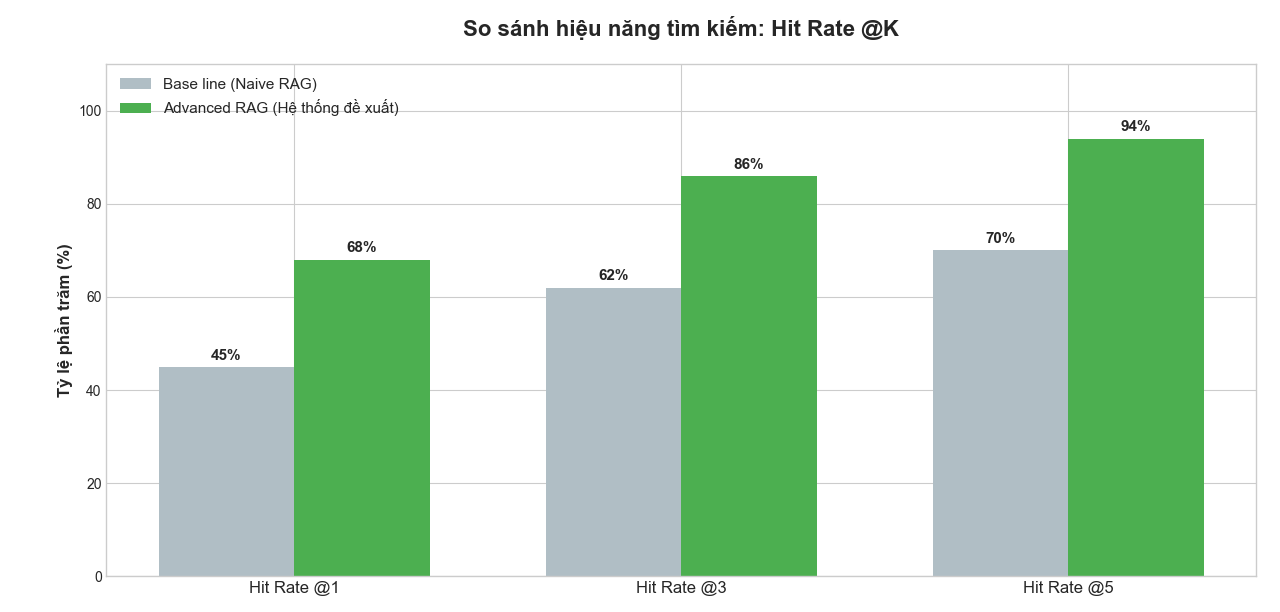
\includegraphics[width=1\textwidth]{images/danhgia1.png}
    \caption{So sánh hiệu năng truy xuất (Hit Rate @K) giữa phương pháp phân mảnh nguyên câu (Naive RAG) và hệ thống đề xuất với chiến lược Parent Document Retrieval (Advanced RAG)}
\end{figure}
Dựa trên tập dữ liệu đánh giá 50 truy vấn (Q\&A pairs), kiến trúc Advanced RAG cho thấy sự cải thiện toàn diện:
\begin{itemize}[leftmargin=*, label={}]
    \item \textbf{Về Hit Rate@K:} Hệ thống Advanced RAG đạt Hit Rate@1 là 68\% và Hit Rate@5 lên tới 94\%, cải thiện vượt bậc so với mức 45\% và 70\% của cấu hình Naive RAG.
    \item \textbf{Về MRR:} Điểm MRR của hệ thống đề xuất dao động dao động trong khoảng từ 0.756 đến 0.790, minh chứng cho việc các đoạn hội thoại chứa đáp án chính xác luôn được bộ tái xếp hạng ưu tiên đẩy lên các vị trí Top đầu.
    \item \textbf{Về Context Relevance:} Do hiệu ứng mở rộng của Cửa sổ trượt, điểm Context Relevance của Advanced RAG có sự sụt giảm nhẹ so với Naive RAG do hệ thống chủ động thu thập thêm các câu thoại lân cận.
\end{itemize}
\textbf{Nhận xét:}
Sự gia tăng đột phá của chỉ số Hit Rate khẳng định hiệu quả cộng hưởng từ chuỗi tối ưu hóa toàn diện của hệ thống Advanced RAG. Trong đó, việc viết lại câu truy vấn giúp xác định chính xác mục tiêu tìm kiếm, chiến lược \textit{Parent Document} giúp giải quyết triệt để điểm yếu cố hữu của Naive RAG là hiện tượng phân mảnh ngữ nghĩa (\textit{semantic fragmentation}). Đặc biệt, sự can thiệp của bộ tái xếp hạng (\textit{Cross-Encoder}) đóng vai trò quyết định trong việc sàng lọc nhiễu và đẩy các dẫn chứng thực sự liên quan lên vị trí ưu tiên, giúp tối ưu hóa chỉ số Hit Rate@1 và MRR. Mặc dù có sự đánh đổi nhỏ về Context Relevance do thu thập thêm một lượng hội thoại phụ trợ xung quanh, đây là sự hy sinh có chủ đích và tối ưu. Lượng thông tin mở rộng từ cơ chế cửa sổ trượt cung cấp đủ luồng giao tiếp (\textit{contextual flow}) làm cơ sở để Mô hình Ngôn ngữ Lớn (LLM) suy luận chính xác đối với các truy vấn phức tạp, loại bỏ hoàn toàn tình trạng đứt gãy thông tin khi chỉ truy xuất các câu thoại đơn lẻ.
\subsection{Đánh giá hiệu quả của siêu dữ liệu (Metadata Filtering)}

\textbf{Vai trò:}
Trong môi trường hội thoại đa diễn giả, việc chỉ dựa vào độ tương đồng ngữ nghĩa (Semantic Search) thuần túy thường dẫn đến sai lệch khi nhiều người cùng thảo luận về một chủ đề bằng các hệ thống từ vựng giống nhau. Siêu dữ liệu (định danh người nói, mốc thời gian) được hệ thống lưu trữ trực tiếp dưới dạng \textit{payload} trong cơ sở dữ liệu vector đóng vai trò như một bộ lọc cứng (\textit{hard filter}). Đánh giá này nhằm xác định mức độ đóng góp của siêu dữ liệu trong việc thu hẹp không gian tìm kiếm và loại bỏ triệt để hiện tượng nhầm lẫn nguồn phát biểu.

\textbf{Thiết lập so sánh:}
\begin{itemize}[leftmargin=*, label={}]
    \item \textbf{Cấu hình cơ sở (Không có Metadata):} Truy xuất tài liệu hoàn toàn dựa trên khoảng cách vector ngữ nghĩa.
    \item \textbf{Cấu hình đề xuất (Có Metadata Filtering):} Kết hợp tìm kiếm vector với kỹ thuật lọc siêu dữ liệu (khoanh vùng theo \textit{Speaker} hoặc khoảng thời gian) trước khi tiến hành tính điểm tương đồng.
\end{itemize}

\textbf{Tiêu chuẩn và Chỉ số đo lường:}
\begin{itemize}[leftmargin=*, label={}]
    \item Khả năng phân luồng và cải thiện độ chính xác truy xuất (đo lường bằng chỉ số \textbf{Hit Rate@K}).
    \item Khả năng đẩy các đoạn hội thoại chứa đáp án của đúng người phát biểu lên vị trí ưu tiên cao nhất (đo lường bằng chỉ số \textbf{MRR}).
\end{itemize}

\textbf{Kết quả thực nghiệm:}
Trên các tập truy vấn đặc thù yêu cầu xác định đích danh chủ thể hành động hoặc thời điểm đưa ra quyết định (ví dụ: "Ai là người đề xuất thêm màn hình hiển thị pin và lo ngại về chi phí?"), việc tích hợp bộ lọc metadata mang lại hiệu quả vượt trội. Cụ thể, hệ thống ghi nhận chỉ số Hit Rate@5 tăng từ 82\% lên 94\%, đồng thời MRR cải thiện từ 0.68 lên 0.76. 

Thực nghiệm cho thấy trong tệp \textit{final\_transcriptions1.json}, khi cả Speaker 1 và Speaker 0 cùng thảo luận về "battery status", hệ thống Naive RAG thường nhầm lẫn giữa người đưa ra ý tưởng (\textit{Speaker 1}: "handy to put a battery status display on it") và người hỏi lại ngữ cảnh (\textit{Speaker 0}: "How much is left in the battery?"). Bằng cách áp dụng bộ lọc \textit{Speaker ID}, hệ thống Advanced RAG đã cô lập chính xác các phát biểu của Speaker 1, từ đó xác định đúng nhân vật này vừa là người đề xuất vừa là người lo ngại về chi phí sản xuất (\textit{drag up the production costs}).

\textbf{Nhận xét:}
Sự gia tăng đồng thời của cả hai chỉ số khẳng định vai trò then chốt của siêu dữ liệu trong việc giải quyết vấn đề chồng lấp từ vựng. Cơ chế \textit{Metadata Filtering} giúp hệ thống bóc tách chính xác các thực thể trong môi trường hội thoại đa người nói vốn có mật độ từ khóa tương đồng rất cao. 

Điều này đặc biệt mang ý nghĩa quyết định đối với các truy vấn về mốc thời gian và phân công nhiệm vụ. Ví dụ, tại tệp \textit{final\_transcriptions4.json}, nếu chỉ tìm kiếm từ khóa "minutes", hệ thống có thể truy xuất nhầm các lượt thảo luận về thời gian họp ở đầu buổi. Tuy nhiên, nhờ siêu dữ liệu thời gian (\textit{start\_time}: 00:34:41), hệ thống đã lọc chính xác lượt phát biểu cuối cuộc họp của Speaker 0 về việc lưu trữ biên bản vào thư mục dự án và giao nhiệm vụ cho nhà thiết kế công nghiệp. Nhờ siêu dữ liệu, Mô hình Ngôn ngữ Lớn (LLM) không còn bị "mù" thông tin chủ thể, đảm bảo câu trả lời luôn được gắn đúng với diễn giả và mốc thời gian thực tế của sự kiện.
\subsection{Đánh giá khả năng tự sửa lỗi của hệ thống RAG}

\textbf{Vai trò:}
Trong điều kiện dữ liệu đầu vào chứa lỗi ASR, hệ thống cần có khả năng phục hồi ngữ nghĩa để đảm bảo kết quả truy xuất và trả lời vẫn chính xác. Đánh giá này nhằm kiểm tra khả năng "tự sửa lỗi" của pipeline RAG.

\textbf{Tiêu chuẩn đánh giá:}
\begin{itemize}
    \item Khả năng hiểu đúng truy vấn khi dữ liệu chứa lỗi chính tả.
    \item Khả năng truy xuất đúng ngữ cảnh dù từ khóa bị biến dạng.
    \item Khả năng chuẩn hóa lại thông tin trong quá trình sinh câu trả lời.
\end{itemize}

\textbf{Chỉ số đo lường:}
\begin{itemize}
    \item HitRate@K trong điều kiện dữ liệu nhiễu
    \item Đánh giá định tính kết quả trả lời
\end{itemize}

\textbf{Kết quả:}
Hệ thống duy trì HitRate@K ở mức \textit{[điền số]} ngay cả khi dữ liệu chứa lỗi ASR. Các trường hợp như ``ô đê a'' → ODA hoặc ``bi hoa xe'' → BIWASE vẫn được xử lý đúng trong phần lớn truy vấn.

\textbf{Nhận xét:}
Cơ chế semantic search đóng vai trò quan trọng trong việc vượt qua lỗi chính tả, trong khi mô hình sinh giúp chuẩn hóa lại thông tin đầu ra. Tuy nhiên, trong các trường hợp lỗi ASR làm thay đổi hoàn toàn ngữ nghĩa, hệ thống vẫn có nguy cơ đưa ra kết quả sai.

\chapter{Kết Luận}

\section{Kết luận}

Đồ án này đã nghiên cứu và đề xuất giải pháp toàn diện cho bài toán khai phá tri thức từ dữ liệu hội thoại đa người nói, đáp ứng nhu cầu cấp thiết về quản trị thông tin trong doanh nghiệp. Bằng việc kết hợp các kỹ thuật tiên tiến trong Xử lý Tiếng nói (Speech Processing) và Xử lý Ngôn ngữ Tự nhiên (NLP), nghiên cứu đã đạt được những đóng góp chính sau:

\begin{itemize}

    \item \textbf{Đánh giá và hoàn thiện pipeline xử lý tiếng nói cho hội thoại đa người nói:} 
    Đồ án đã tiến hành phân tích và đánh giá có hệ thống các cấu hình xử lý tiếng nói trong bài toán hội thoại đa người nói, bao gồm lựa chọn mô hình embedding (ECAPA-TDNN, TitaNet-Large), thuật toán phân cụm (Spectral Clustering, AHC) và chiến lược phân tích một lớp và hai lớp. Kết quả thực nghiệm cho thấy Spectral Clustering kết hợp embedding dựa trên ECAPA/TitaNet đạt hiệu năng ổn định, với chỉ số Confusion giảm và Quality cao, đồng thời DER nằm trong mức cạnh tranh so với các hệ thống diarization hiện đại được báo cáo trong các benchmark gần đây. Việc mở rộng sang cấu hình hai lớp phân tích giúp cải thiện rõ rệt Quality và giảm Confusion, đặc biệt tại các ranh giới hội thoại phức tạp, qua đó nâng cao độ tin cậy của pipeline diarization phục vụ trực tiếp cho ASR ở các bước xử lý tiếp theo.

    \item \textbf{Thiết lập quy trình xử lý tiếng nói tích hợp (Integrated Speech Pipeline):} 
    Nghiên cứu đã xây dựng thành công kiến trúc đường ống kết hợp chặt chẽ giữa mô-đun Phân đoạn người nói (Speaker Diarization) dựa trên thuật toán Phân cụm phổ (Spectral Clustering) và mô hình nhận dạng tiếng nói tự động (ASR). Kết quả thực nghiệm cho thấy hệ thống có khả năng chuyển đổi hiệu quả dữ liệu âm thanh phi cấu trúc thành văn bản có cấu trúc, bảo toàn tính toàn vẹn về định danh người nói và tham chiếu thời gian.

    \item \textbf{Tối ưu hóa kiến trúc RAG cho dữ liệu hội thoại:} 
    Đồ án đã triển khai thành công mô hình \textit{Retrieval-Augmented Generation} (RAG) chuyên biệt hóa, tận dụng sức mạnh của cơ sở dữ liệu vector Qdrant và chiến lược Tái xếp hạng (Re-ranking). Phương pháp này đã giải quyết triệt để vấn đề "ảo giác" (hallucination) của các Mô hình Ngôn ngữ Lớn (LLM), đảm bảo thông tin đầu ra có tính xác thực cao và được neo giữ (\textit{grounded}) chặt chẽ vào ngữ cảnh biên bản gốc.

    \item \textbf{Chứng minh tính bền vững trên dữ liệu nhiễu (Robustness on Noisy Data):} 
    Thông qua kiểm thử thực nghiệm trên tập dữ liệu chuyên ngành cấp thoát nước (BIWASE), hệ thống thể hiện khả năng vượt trội trong việc trích xuất chính xác các thực thể quan trọng (số liệu tài chính, mốc thời gian) ngay cả khi dữ liệu đầu vào chịu ảnh hưởng bởi nhiễu sai số từ mô hình ASR. Điều này khẳng định khả năng hiểu ngữ nghĩa (Semantic Understanding) của hệ thống thay vì chỉ so khớp từ khóa đơn thuần.

    \item \textbf{Nâng cao trải nghiệm tương tác ngữ cảnh (Context-Aware Interaction):} 
    Hệ thống đã tích hợp thành công cơ chế quản lý trạng thái hội thoại và viết lại câu truy vấn (Query Rewriting). Tính năng này cho phép duy trì mạch hội thoại đa lượt một cách tự nhiên, hỗ trợ người dùng truy xuất thông tin phức tạp thông qua giao diện hỏi đáp trực quan, thay thế phương thức tìm kiếm từ khóa truyền thống.
\end{itemize}

\subsection{Những hạn chế}
Mặc dù hệ thống đạt được hiệu năng ổn định trong các kịch bản thực nghiệm, nghiên cứu vẫn tồn tại một số hạn chế. Thứ nhất, pipeline xử lý tiếng nói phụ thuộc mạnh vào chất lượng của ASR; các lỗi nhận dạng từ vựng và ranh giới câu có thể lan truyền sang các bước gán nhãn và truy xuất. Thứ hai, quá trình đánh giá diarization chủ yếu dựa trên các chỉ số tổng hợp như DER, Miss và Confusion, trong khi chưa có đánh giá định lượng trực tiếp về tác động của từng loại lỗi lên chất lượng truy xuất cuối cùng. Thứ ba, việc sử dụng mô hình ngôn ngữ lớn để hiệu chỉnh cấu trúc hội thoại hiện mới dừng ở mức thực nghiệm, chưa có cơ chế đánh giá tự động và chưa đảm bảo tính ổn định trong mọi ngữ cảnh. Cuối cùng, phạm vi thí nghiệm còn giới hạn về ngôn ngữ, môi trường âm thanh và quy mô phần cứng, do đó kết quả chưa thể khái quát cho các kịch bản hội thoại đa miền hoặc triển khai ở quy mô lớn.

Bên cạnh những kết quả khả quan bước đầu, mô-đun RAG hiện tại vẫn tồn tại một số hạn chế cần được khắc phục trong các nghiên cứu tiếp theo. Thứ nhất, chiến lược phân đoạn dữ liệu (\textit{chunking}) dựa trên từng câu thoại đơn lẻ kết hợp với cơ chế mở rộng ngữ cảnh cố định (lấy $\pm 1$ câu lân cận) đôi khi chưa bao quát trọn vẹn ý nghĩa trong các luồng thảo luận dài và phức tạp, dẫn đến rủi ro đứt gãy ngữ nghĩa. Thứ hai, quá trình đánh giá hiện mới chỉ dừng lại ở phương pháp định tính thông qua các kịch bản kiểm thử (\textit{Case Studies}) do thiếu bộ dữ liệu nhãn chuẩn (\textit{Ground Truth}) để đo lường cụ thể các chỉ số hiệu năng như độ chính xác ngữ cảnh (\textit{Context Precision}) hay độ phủ thông tin (\textit{Recall}). Cuối cùng, hệ thống vẫn chịu ảnh hưởng bởi sự lan truyền lỗi từ đầu vào ASR và độ trễ xử lý còn khá cao do quy trình thực thi tuần tự qua nhiều bước (viết lại câu hỏi, tìm kiếm vector và tái xếp hạng) chưa được tối ưu hóa cho các ứng dụng thời gian thực.


\subsection{Định hướng phát triển}

Trong các hướng mở rộng của hệ thống, việc khai thác và tổ chức \textbf{metadata} đóng vai trò then chốt nhằm nâng cao hiệu quả truy xuất và tổng hợp thông tin. Cụ thể, hệ thống có thể được mở rộng theo các hướng sau:

\begin{itemize}
    \item \textbf{Bổ sung metadata giàu ngữ cảnh:}
    Mỗi đoạn hội thoại được gắn thêm các trường chỉ mục như tên tệp âm thanh, ngày–giờ cuộc họp, chủ đề ước lượng, tóm tắt ngắn theo đoạn hoặc theo cụm người nói. Các metadata này cho phép kết hợp truy vấn ngữ nghĩa với lọc điều kiện (metadata filtering), giúp thu hẹp không gian tìm kiếm một cách hiệu quả.
    \item \textbf{Chỉ mục phân cấp (Hierarchical Indexing):} Thay vì lưu trữ các đoạn hội thoại độc lập, hệ thống có thể xây dựng chỉ mục theo nhiều mức: cuộc họp $\rightarrow$ người nói $\rightarrow$ đoạn hội thoại. Cấu trúc này hỗ trợ tốt hơn cho các truy vấn dạng “ai nói gì, ở cuộc họp nào, vào thời điểm nào”.
    \item \textbf{Tối ưu embedding cho truy xuất:}
    Việc sử dụng các mô hình embedding nhẹ hơn (ví dụ MiniLM) cho các trường metadata và tóm tắt giúp giảm chi phí lưu trữ và tăng tốc độ truy vấn, trong khi vẫn giữ các embedding giàu ngữ nghĩa cho nội dung hội thoại chính.

    \item \textbf{Mở rộng chiến lược lưu trữ vector:}
    Cơ sở dữ liệu vector có thể được cấu hình để tách riêng embedding nội dung và embedding metadata, kết hợp với cơ chế re-ranking dựa trên metadata nhằm cải thiện độ chính xác của kết quả truy xuất trong các tập dữ liệu lớn.
\end{itemize}
\printbibliography
% \input{sections/references}

% \input{sections/appendixes/appendix}
% \input{sections/appendixes/plan}
% % add appendix later on

\end{document}
